
 
  %%%% NEW D/I


\begin{figure}
  \begin{center}
  \begin{tabular}{m{8ex}m{\kernelfigwidth}m{\kernelfigwidth}|m{\kernelfigwidth}m{\kernelfigwidth}}
$b=90^\circ$&
\hspace{\kernelfigspace}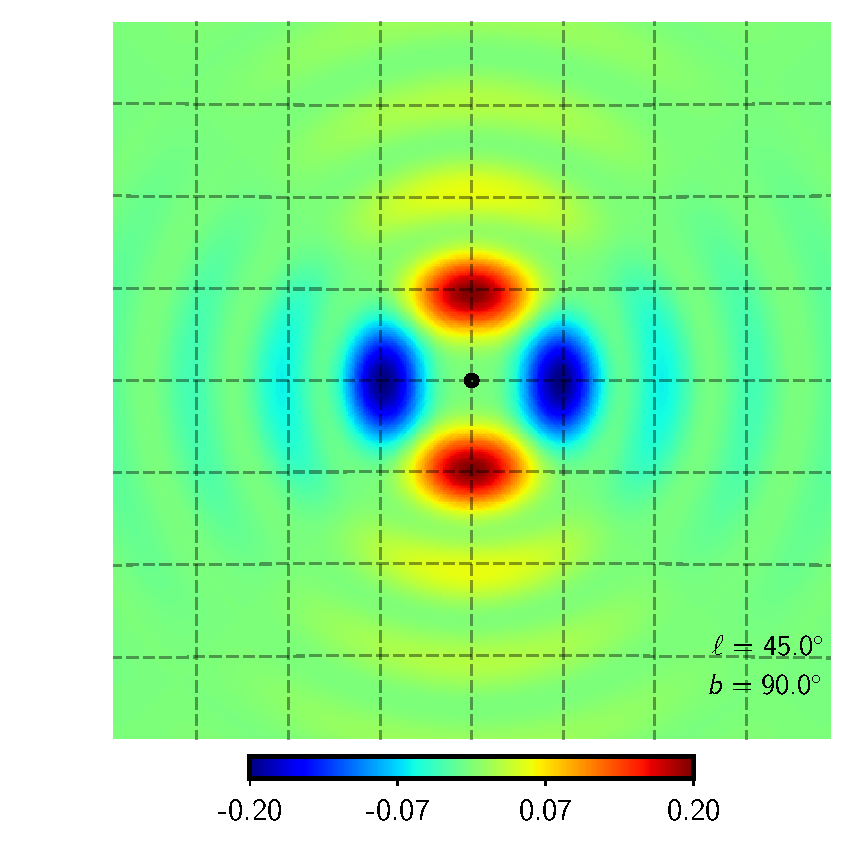
\includegraphics[width=\kernelfigwidth]{new_kernel/qu2ebqu_rker_D_lat90_lon45.pdf} &
\hspace{\kernelfigspace}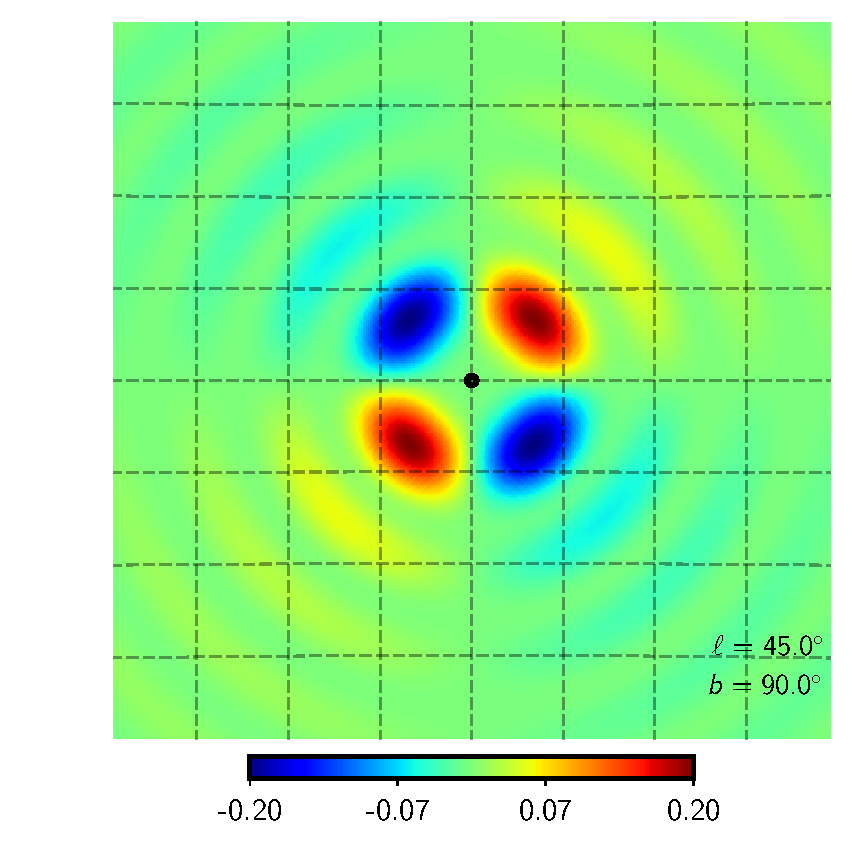
\includegraphics[width=\kernelfigwidth]{new_kernel/qu2ebqu_iker_D_lat90_lon45.pdf} &
\hspace{\kernelfigspace}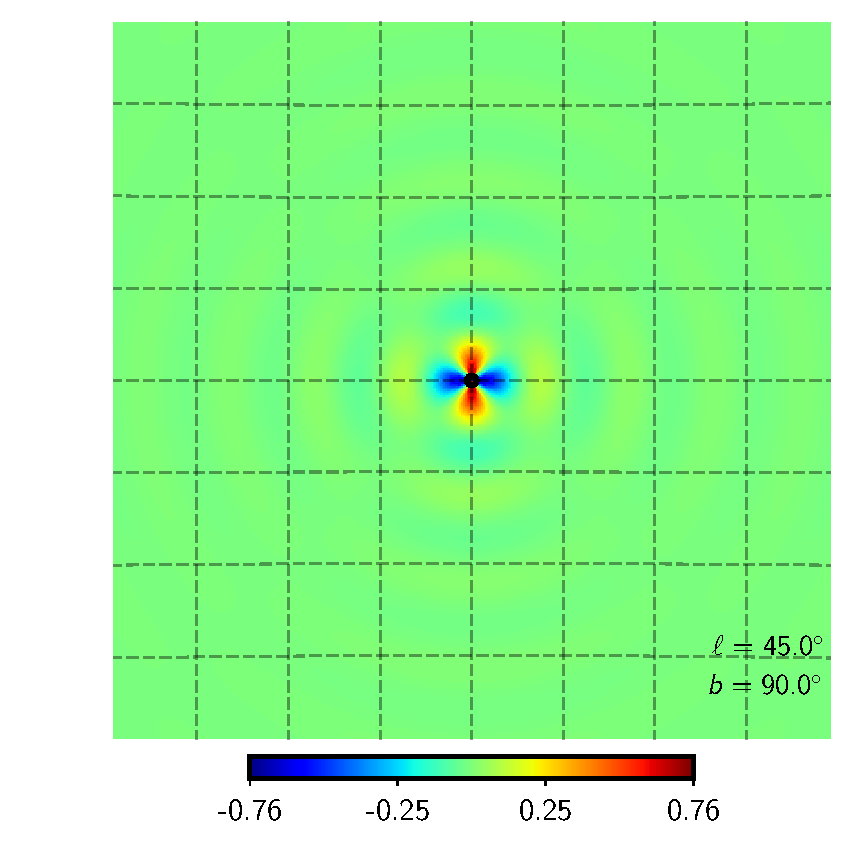
\includegraphics[width=\kernelfigwidth]{new_kernel/qu2ebqu_rker_I_lat90_lon45.pdf} &
\hspace{\kernelfigspace}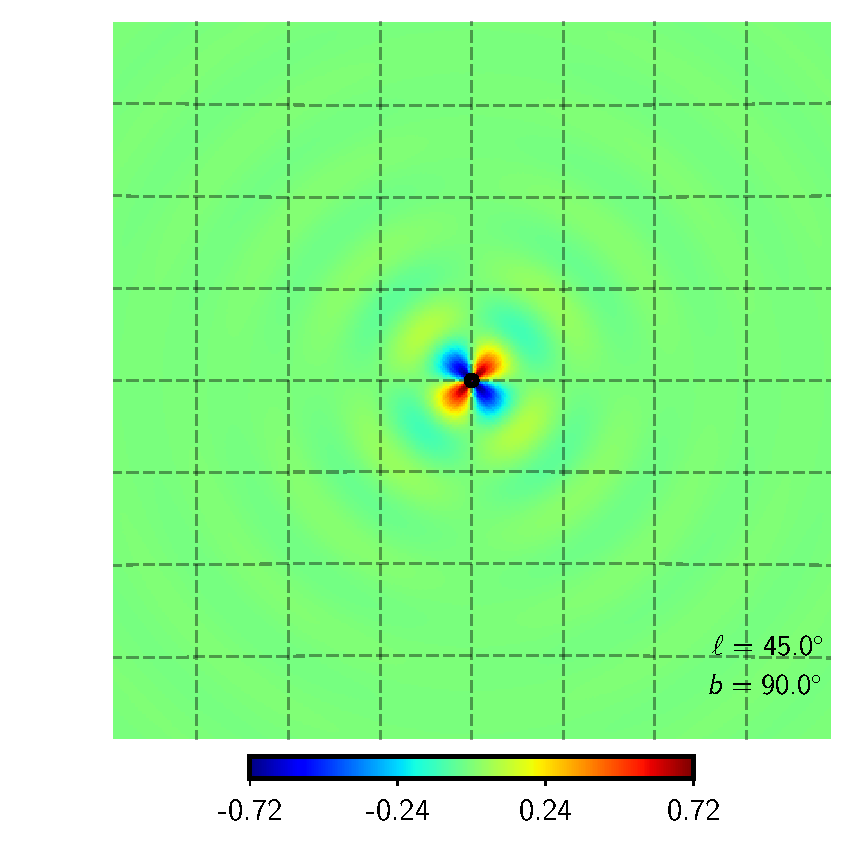
\includegraphics[width=\kernelfigwidth]{new_kernel/qu2ebqu_iker_I_lat90_lon45.pdf} \\
$b=87^\circ$&
\hspace{\kernelfigspace}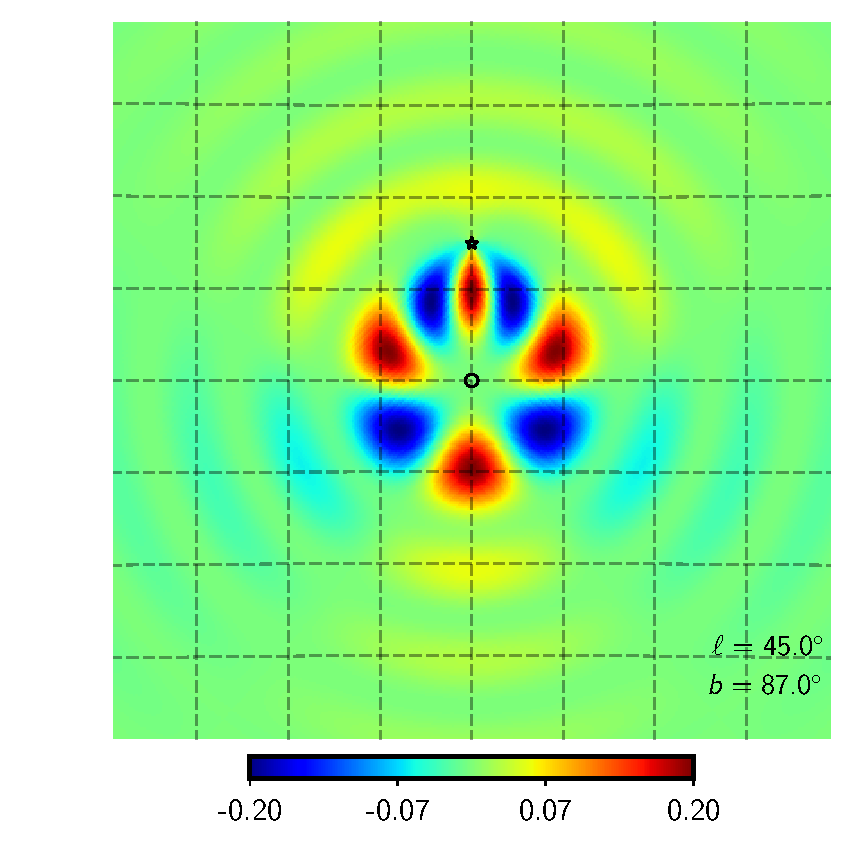
\includegraphics[width=\kernelfigwidth]{new_kernel/qu2ebqu_rker_D_lat87_lon45.pdf} &
\hspace{\kernelfigspace}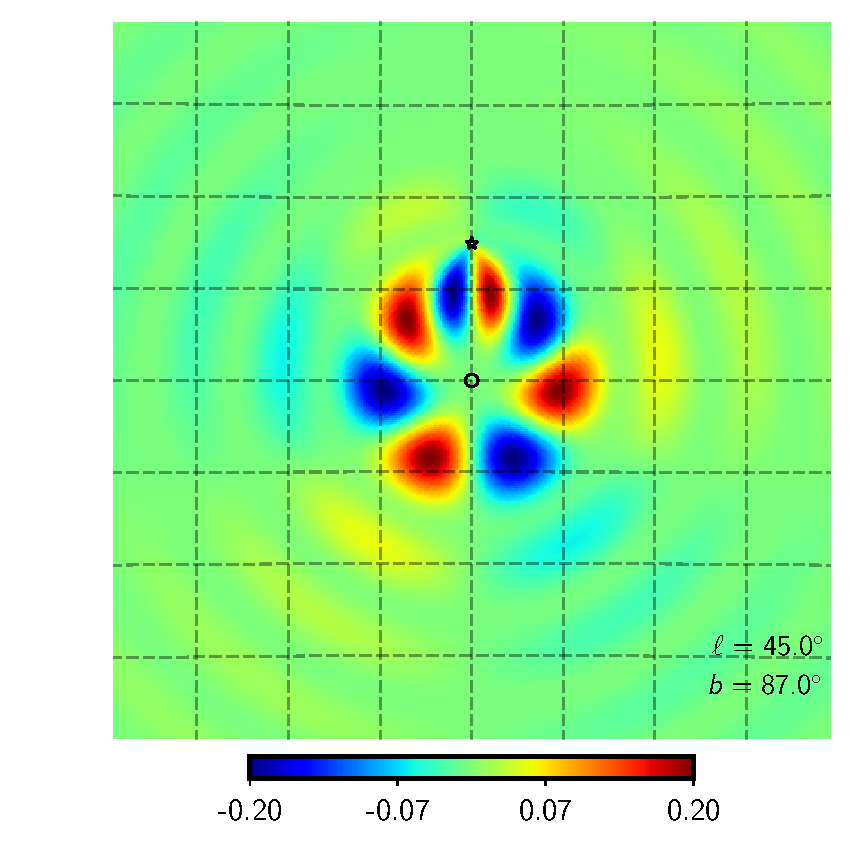
\includegraphics[width=\kernelfigwidth]{new_kernel/qu2ebqu_iker_D_lat87_lon45.pdf} &
\hspace{\kernelfigspace}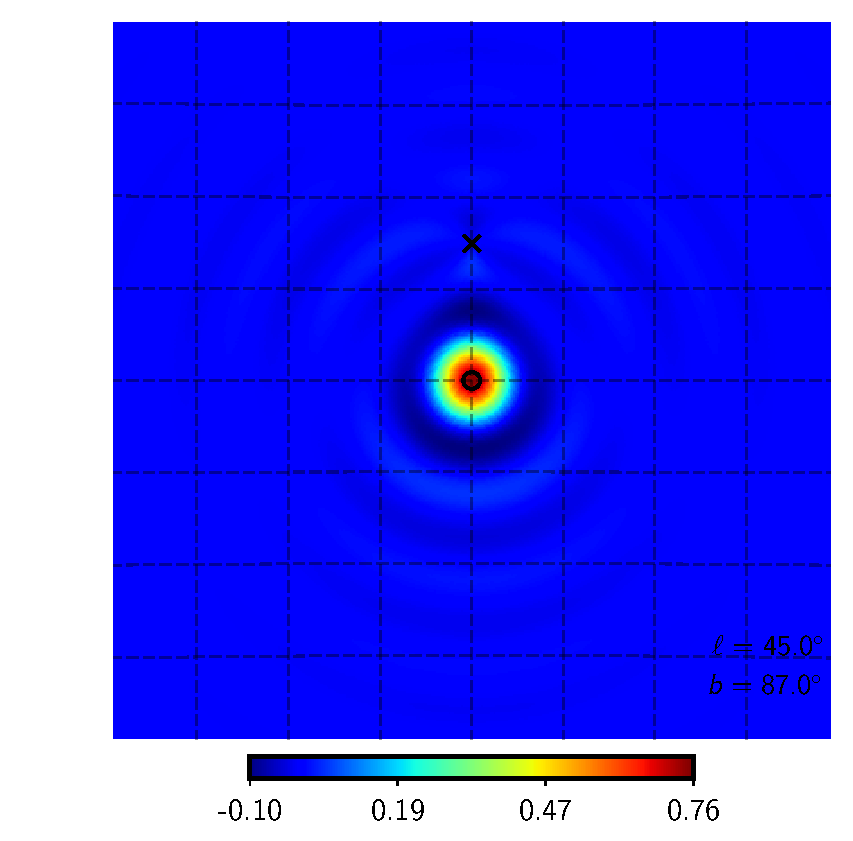
\includegraphics[width=\kernelfigwidth]{new_kernel/qu2ebqu_rker_I_lat87_lon45.pdf} &
\hspace{\kernelfigspace}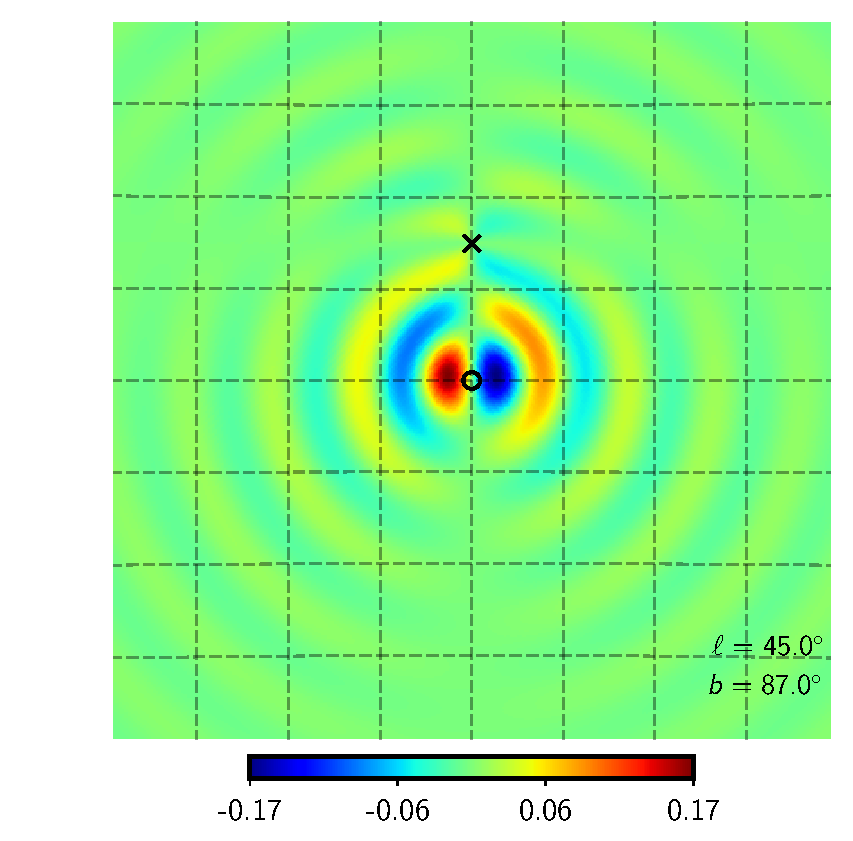
\includegraphics[width=\kernelfigwidth]{new_kernel/qu2ebqu_iker_I_lat87_lon45.pdf} \\
$b=80^\circ$&
\hspace{\kernelfigspace}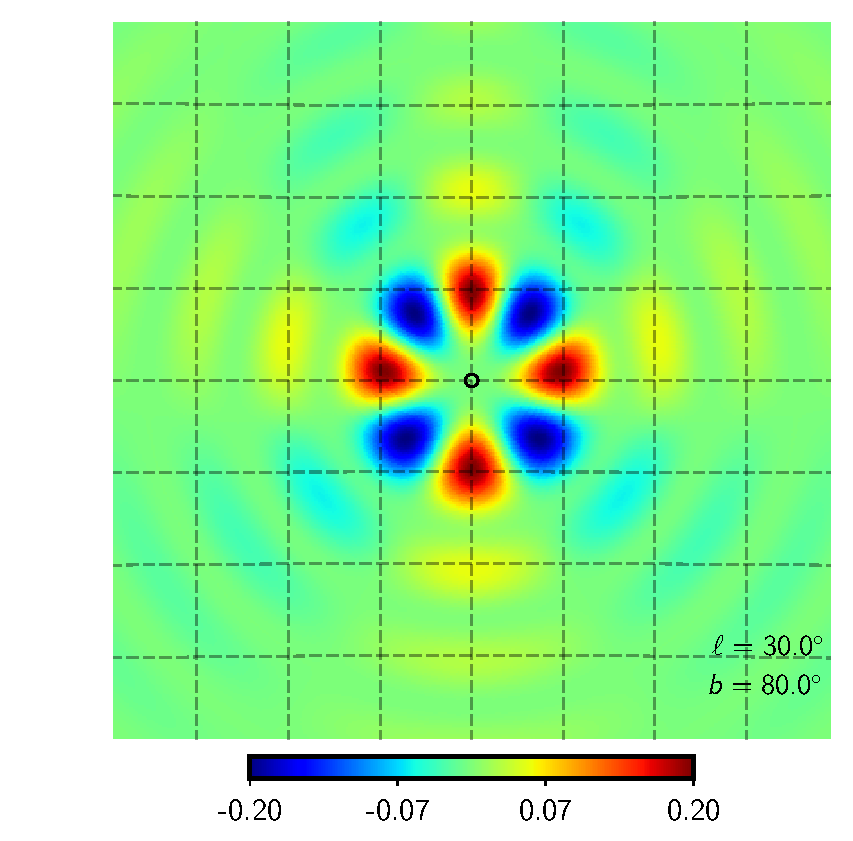
\includegraphics[width=\kernelfigwidth]{new_kernel/qu2ebqu_rker_D_lat80_lon30.pdf} &
\hspace{\kernelfigspace}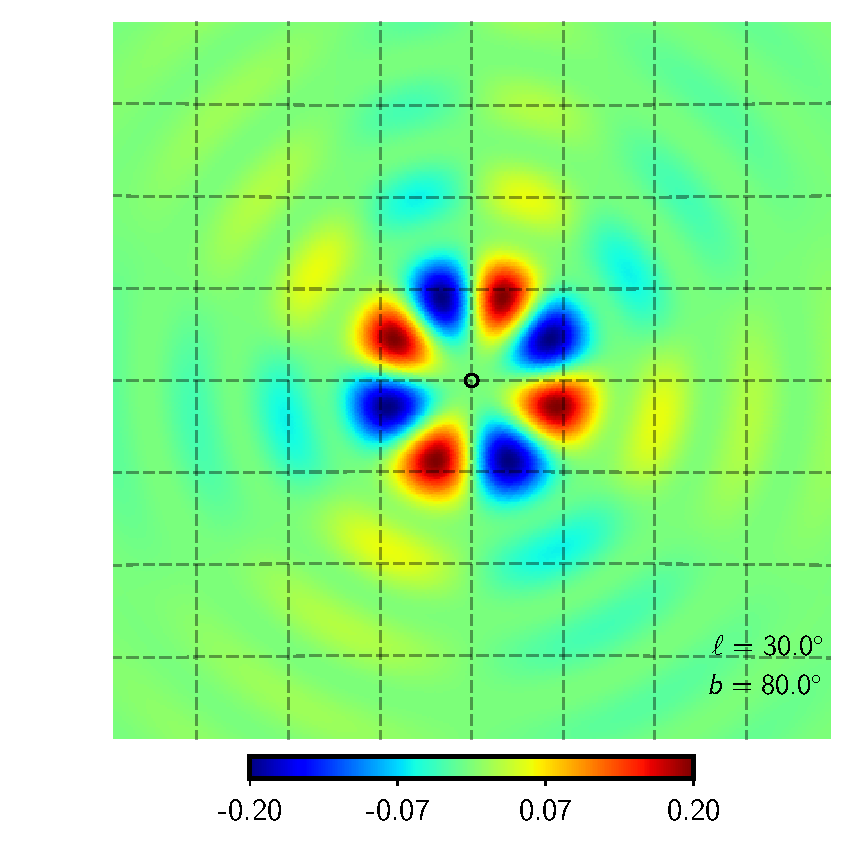
\includegraphics[width=\kernelfigwidth]{new_kernel/qu2ebqu_iker_D_lat80_lon30.pdf} &
\hspace{\kernelfigspace}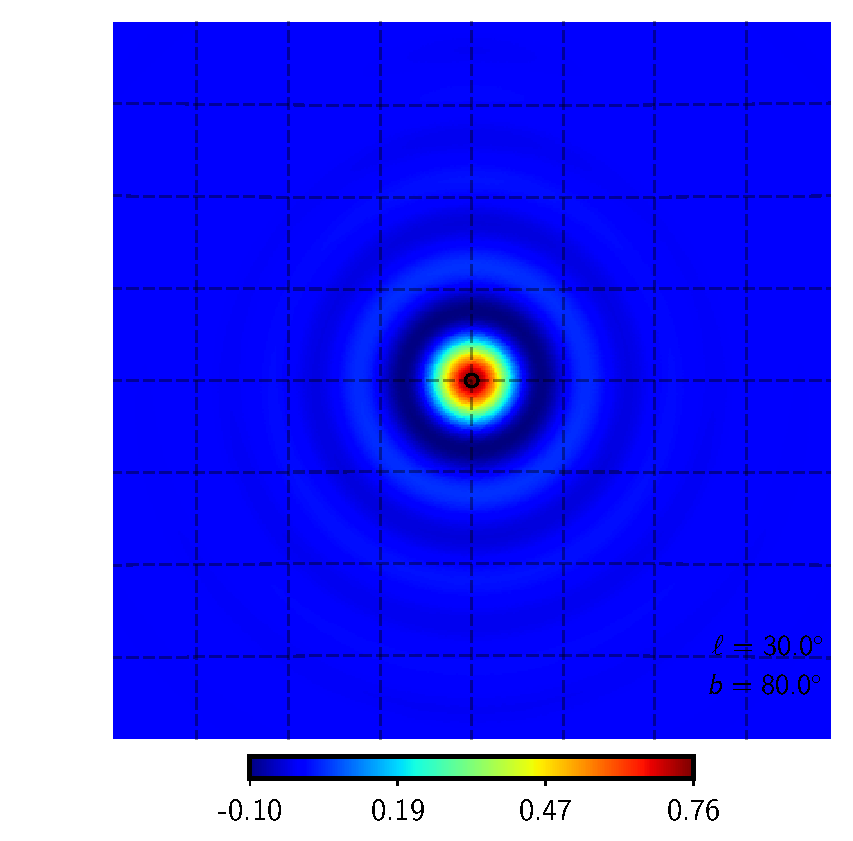
\includegraphics[width=\kernelfigwidth]{new_kernel/qu2ebqu_rker_I_lat80_lon30.pdf} &
\hspace{\kernelfigspace}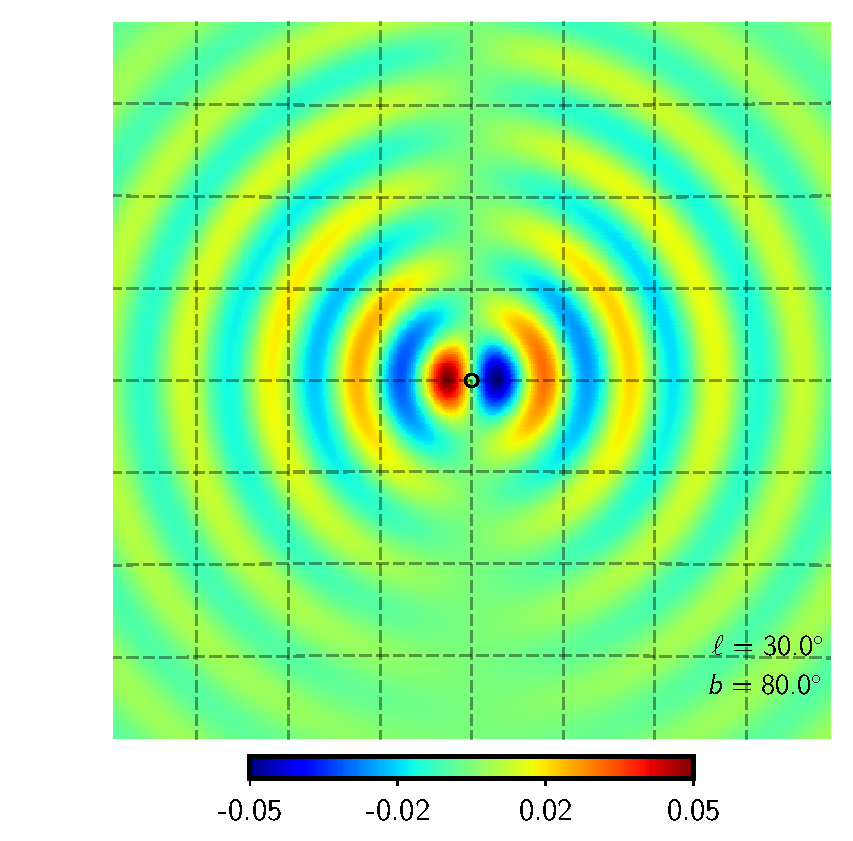
\includegraphics[width=\kernelfigwidth]{new_kernel/qu2ebqu_iker_I_lat80_lon30.pdf} \\
$b=0^\circ$&
\hspace{\kernelfigspace}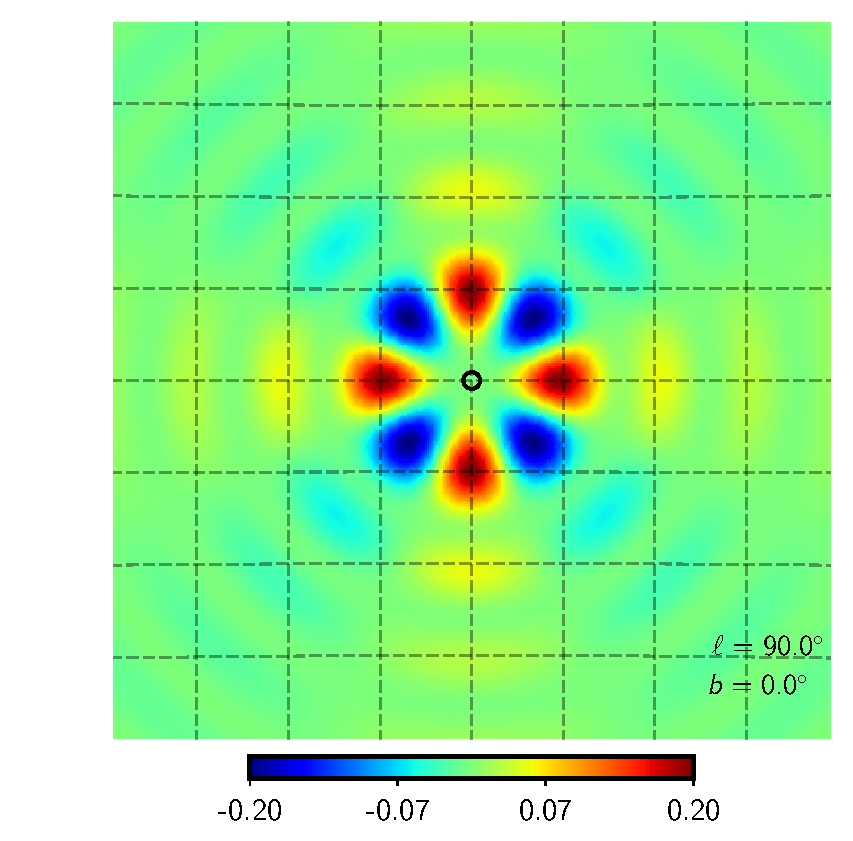
\includegraphics[width=\kernelfigwidth]{new_kernel/qu2ebqu_rker_D_lat0_lon90.pdf} &
\hspace{\kernelfigspace}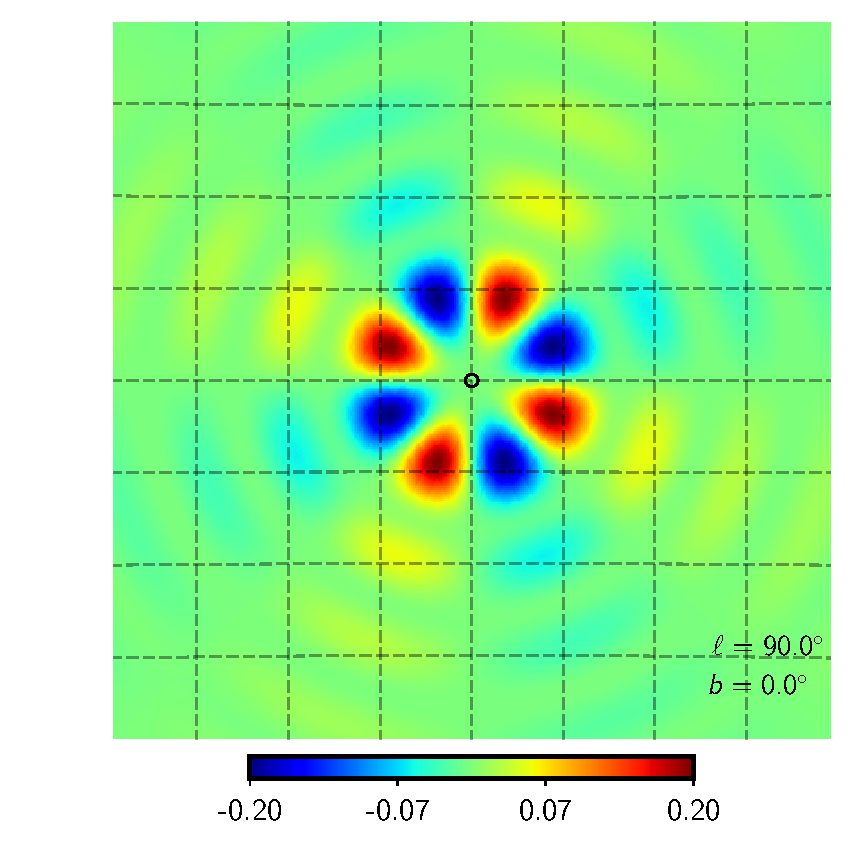
\includegraphics[width=\kernelfigwidth]{new_kernel/qu2ebqu_iker_D_lat0_lon90.pdf} &
\hspace{\kernelfigspace}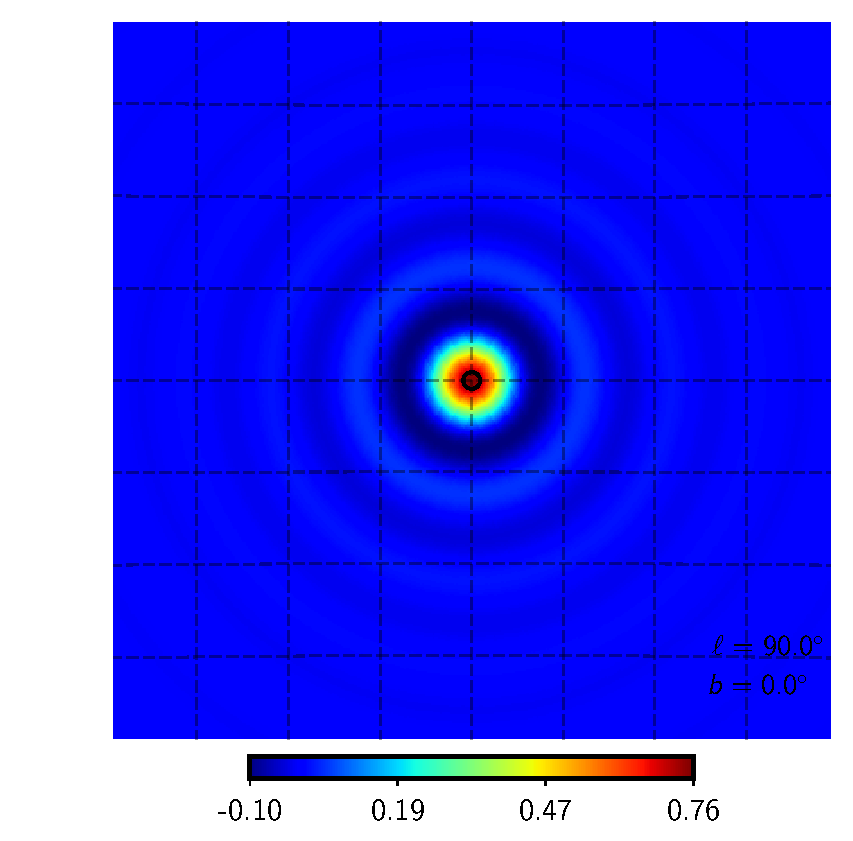
\includegraphics[width=\kernelfigwidth]{new_kernel/qu2ebqu_rker_I_lat0_lon90.pdf} &
\hspace{\kernelfigspace}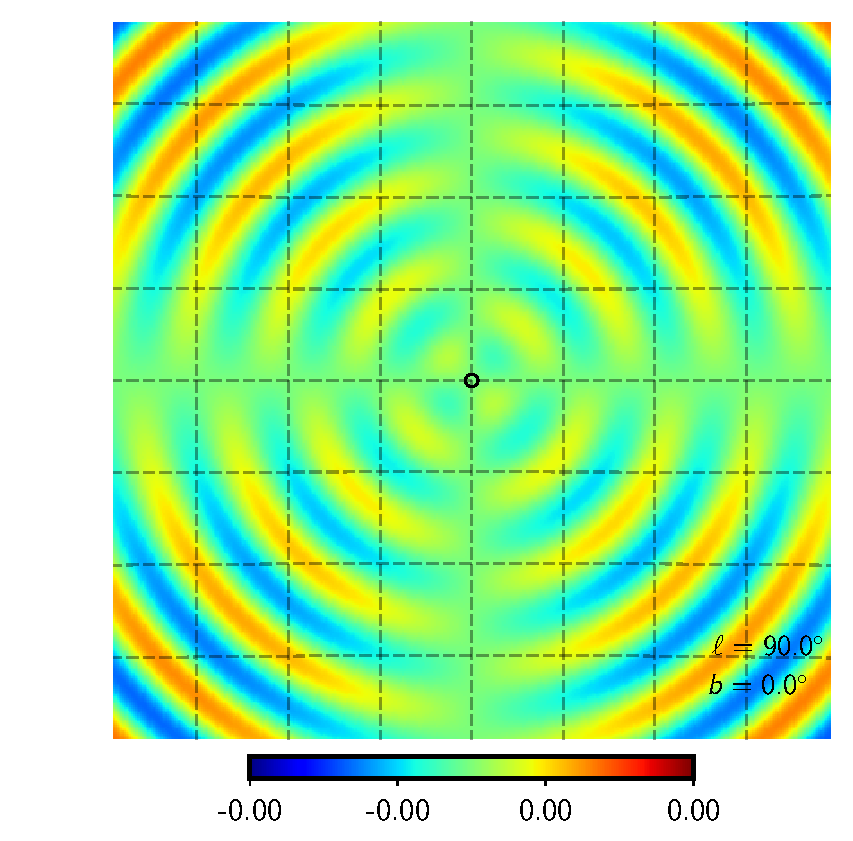
\includegraphics[width=\kernelfigwidth]{new_kernel/qu2ebqu_iker_I_lat0_lon90.pdf} \\
&
\centering $\textrm{Re} \left(\mathcal{D} \right)$ &
\centering $\textrm{Im} \left(\mathcal{D} \right)$ &
\centering $\textrm{Re} \left(\mathcal{I} \right)$ &
\centering $\textrm{Im} \left(\mathcal{I} \right)$
  \end{tabular}
  \end{center}
  \caption{Like Figure \ref{fig:vis_kernel}, but for the kernels that purify Stokes parameter into their $E/B$ parts.} \label{fig:vis_kernel_DI}
\end{figure}

%\begin{figure} \label{fig:mixing_kernel}
  %%%%  OLD VERSION %%%%
%  \centering
%\captionsetup[subfigure]{labelformat=empty}
%\subfigure{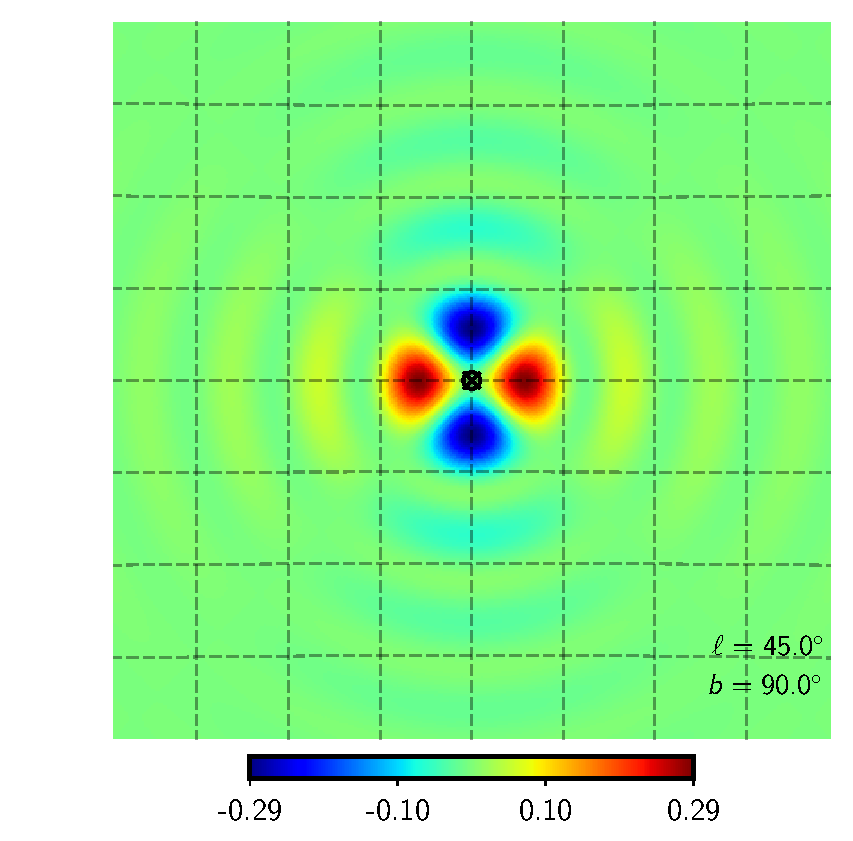
\includegraphics[width=0.125\columnwidth]{new_kernel/qu2eb_rker_rad_lat90_lon45.pdf}}\hspace{-2mm}
%\subfigure{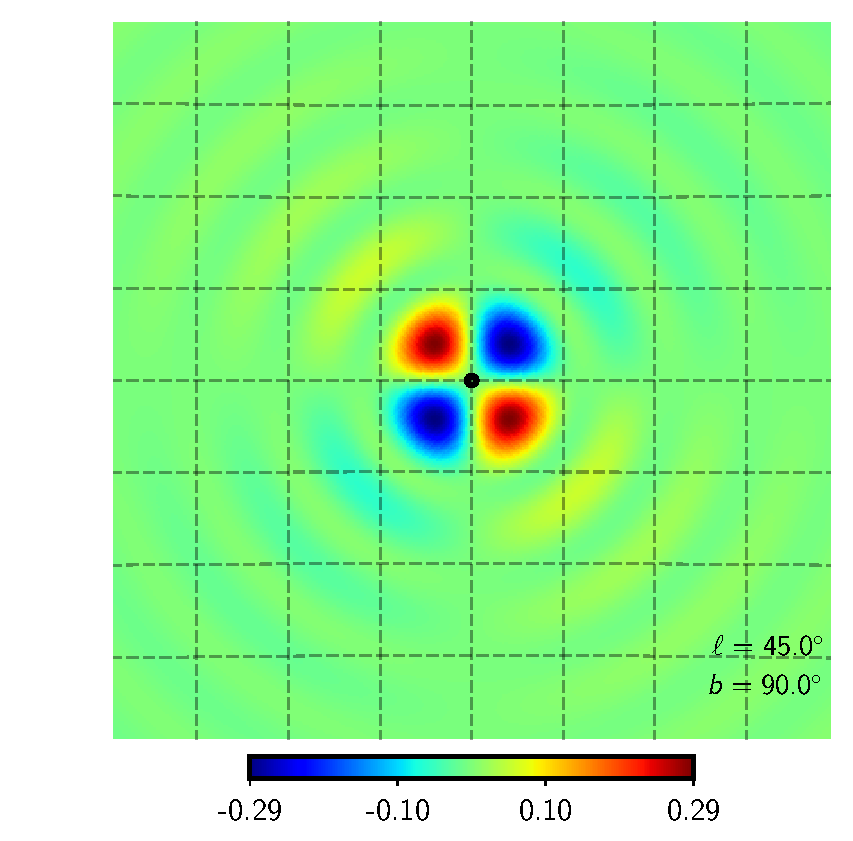
\includegraphics[width=0.125\columnwidth]{new_kernel/qu2eb_iker_rad_lat90_lon45.pdf}}\hspace{-2mm}
%\subfigure{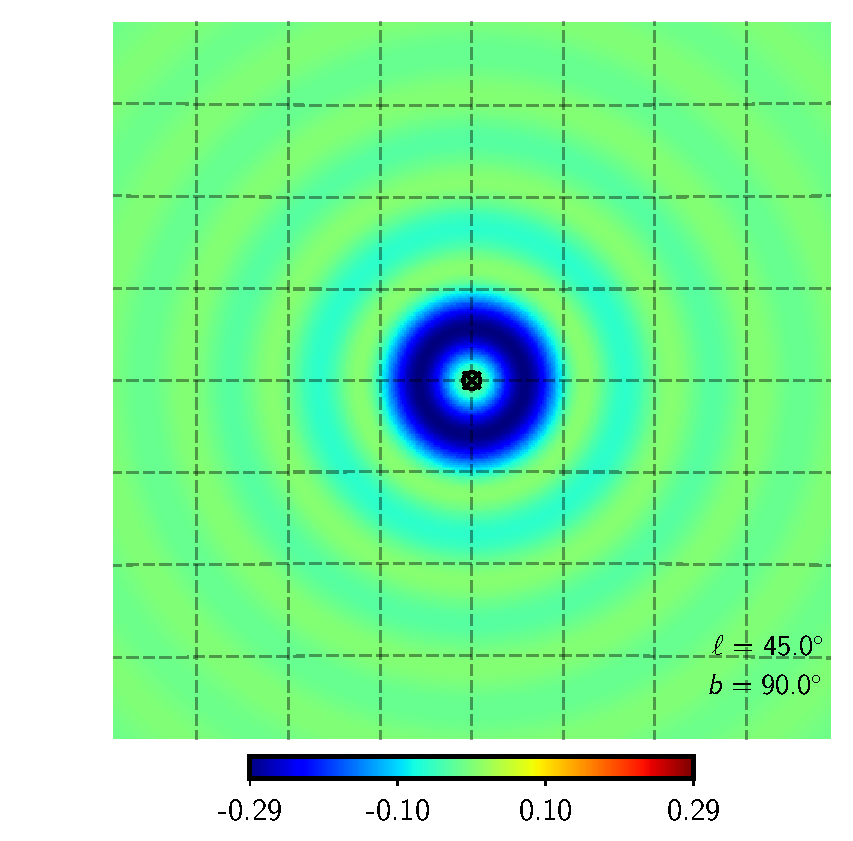
\includegraphics[width=0.125\columnwidth]{new_kernel/qu2eb_rker_con_lat90_lon45.pdf}}\hspace{-2mm}
%\subfigure{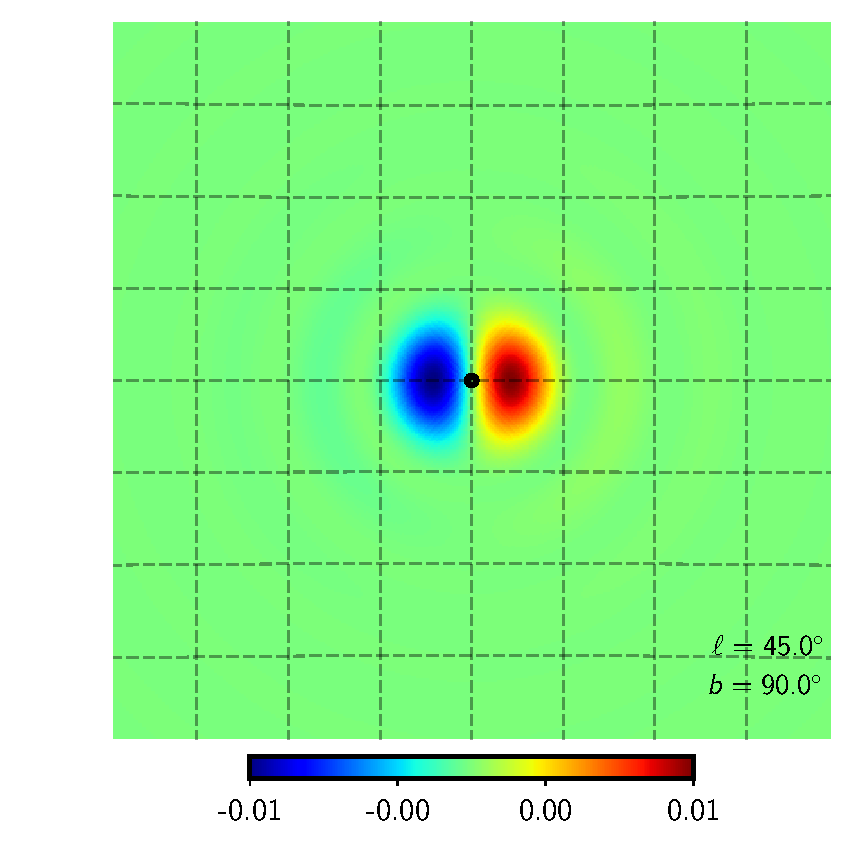
\includegraphics[width=0.125\columnwidth]{new_kernel/qu2eb_iker_con_lat90_lon45.pdf}}\hspace{-2mm}
%\subfigure{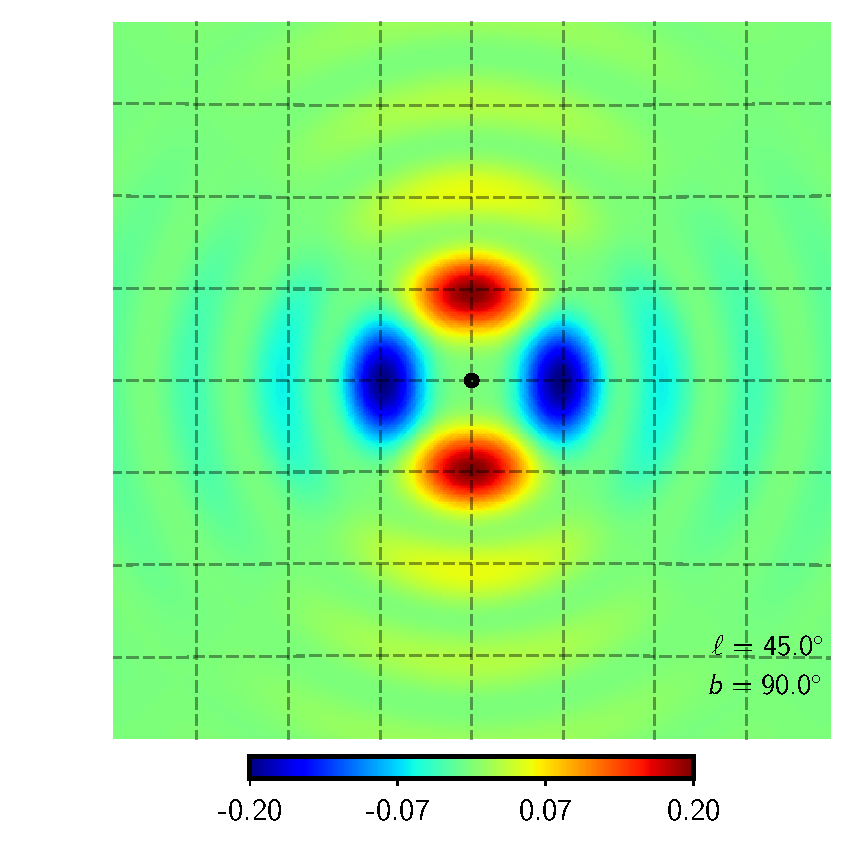
\includegraphics[width=0.125\columnwidth]{new_kernel/qu2ebqu_rker_D_lat90_lon45.pdf}}\hspace{-2mm}
%\subfigure{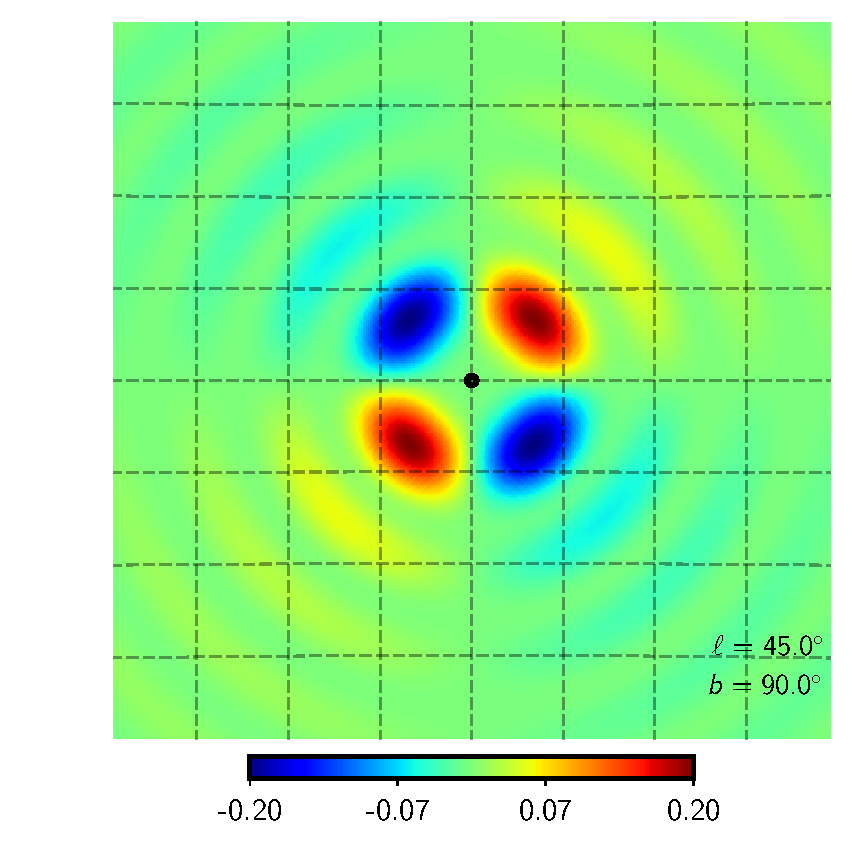
\includegraphics[width=0.125\columnwidth]{new_kernel/qu2ebqu_iker_D_lat90_lon45.pdf}}\hspace{-2mm}
%\subfigure{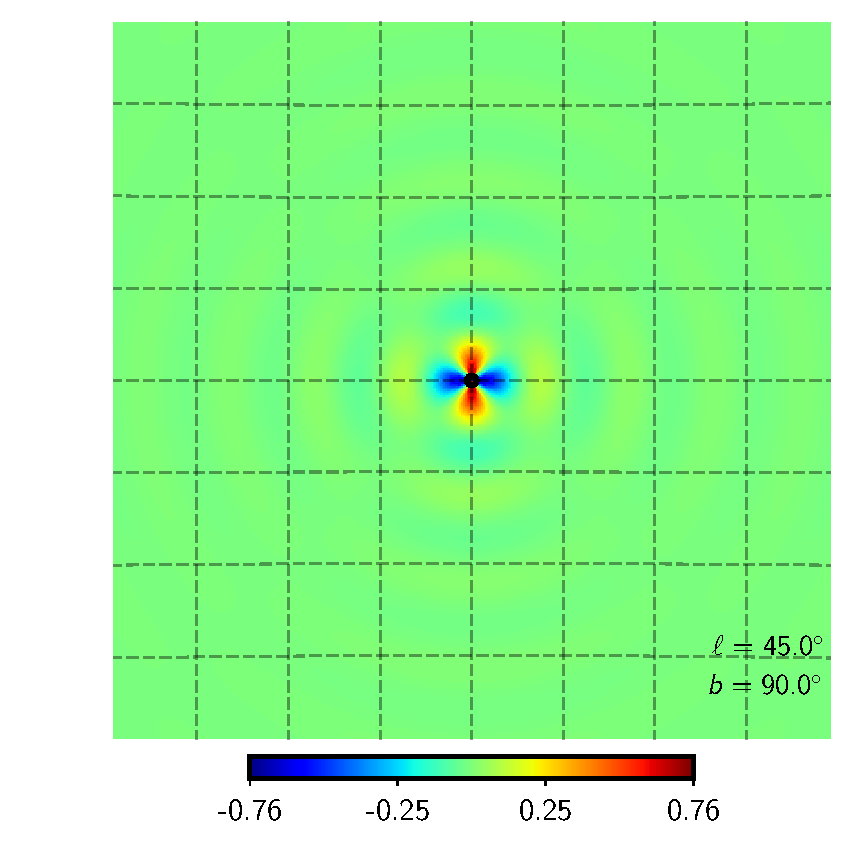
\includegraphics[width=0.125\columnwidth]{new_kernel/qu2ebqu_rker_I_lat90_lon45.pdf}}\hspace{-2mm}
%\subfigure{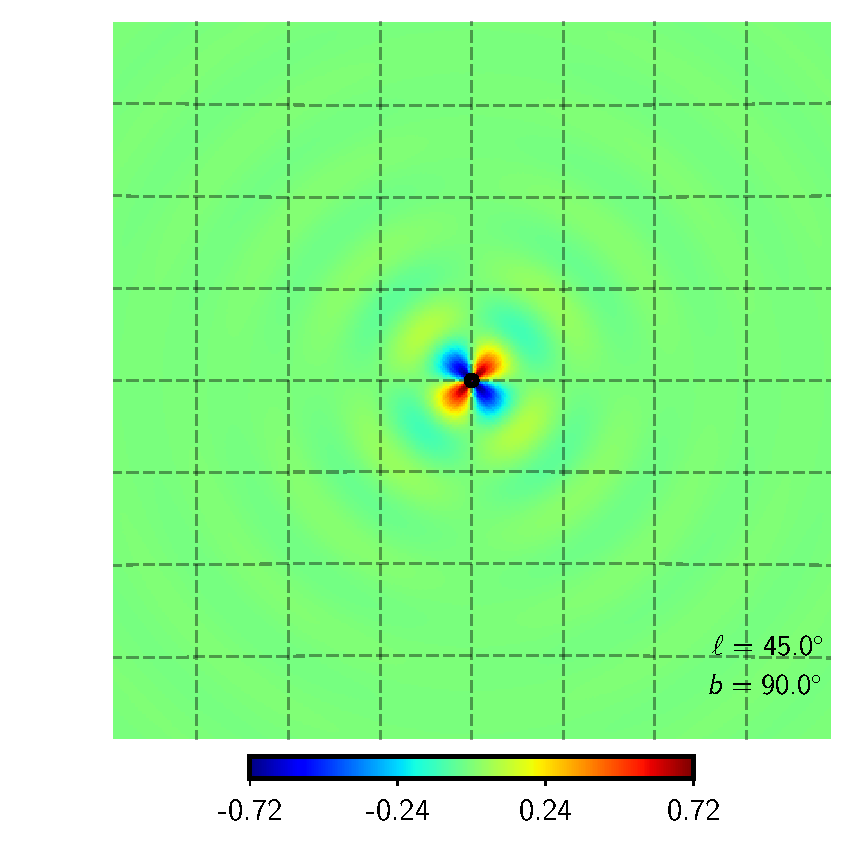
\includegraphics[width=0.125\columnwidth]{new_kernel/qu2ebqu_iker_I_lat90_lon45.pdf}}\hspace{-2mm}

%\subfigure{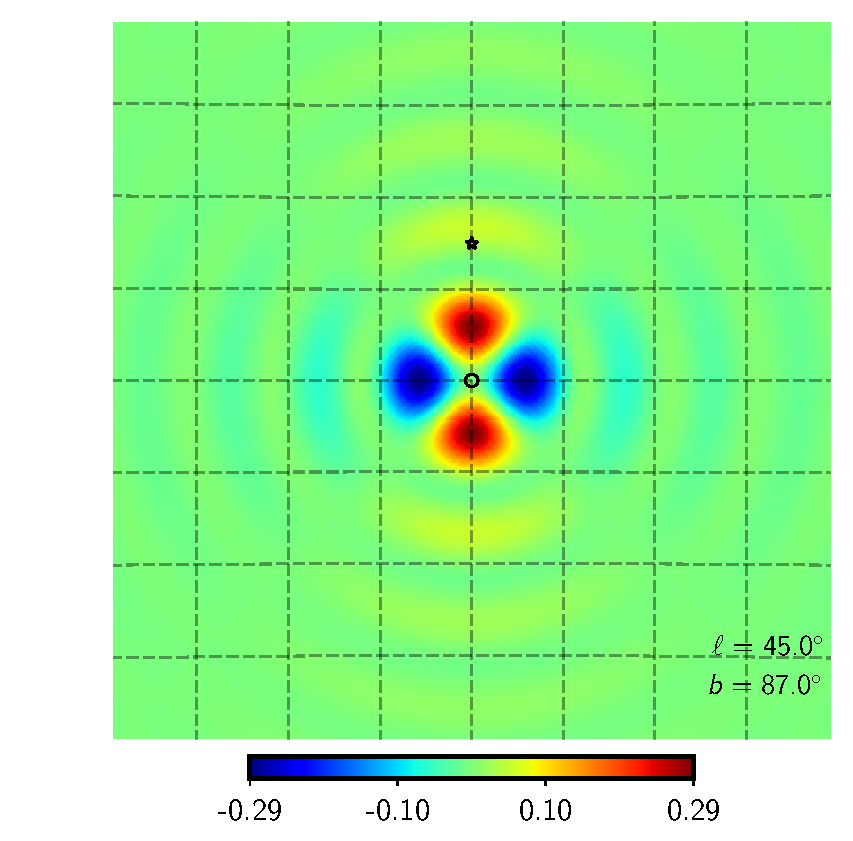
\includegraphics[width=0.125\columnwidth]{new_kernel/qu2eb_rker_rad_lat87_lon45.pdf}}\hspace{-2mm}
%\subfigure{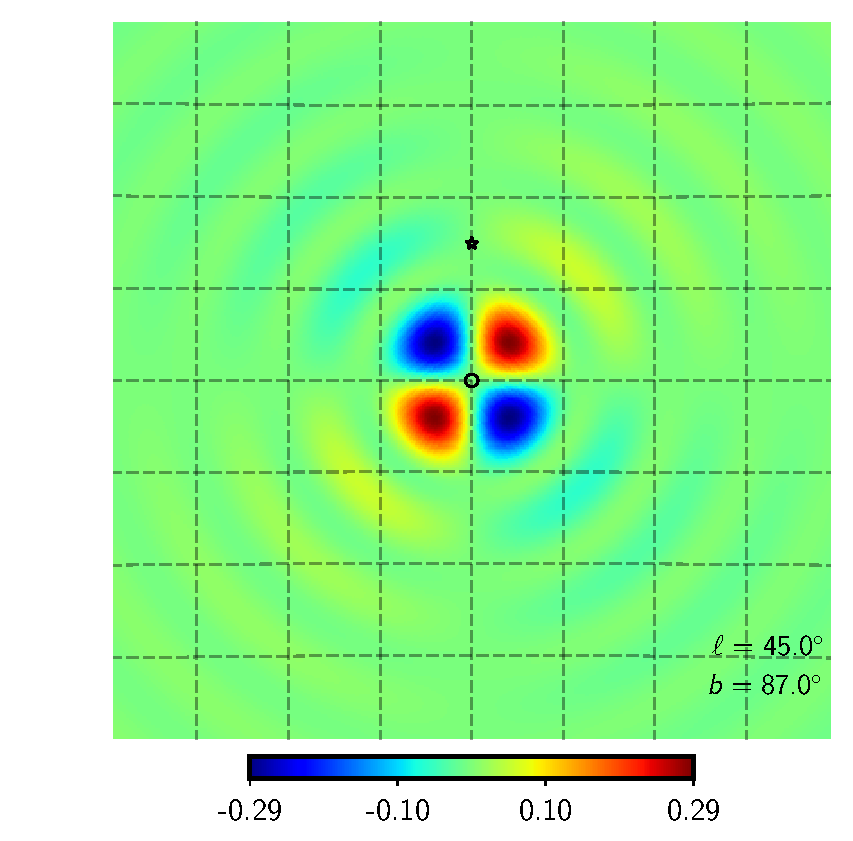
\includegraphics[width=0.125\columnwidth]{new_kernel/qu2eb_iker_rad_lat87_lon45.pdf}}\hspace{-2mm}
%\subfigure{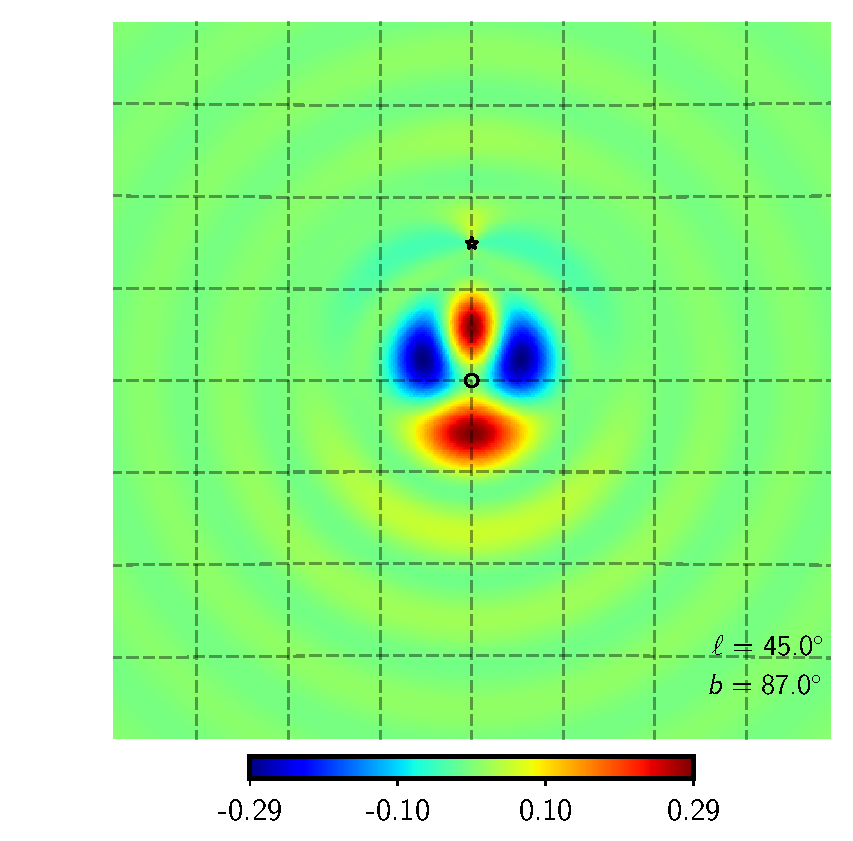
\includegraphics[width=0.125\columnwidth]{new_kernel/qu2eb_rker_con_lat87_lon45.pdf}}\hspace{-2mm}
%\subfigure{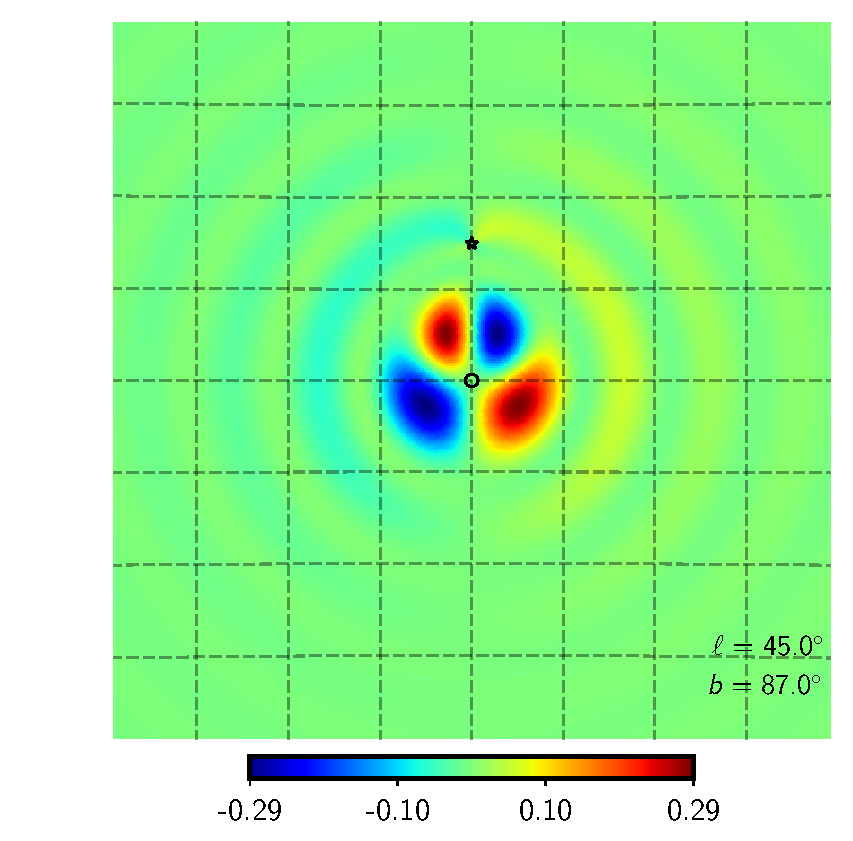
\includegraphics[width=0.125\columnwidth]{new_kernel/qu2eb_iker_con_lat87_lon45.pdf}}\hspace{-2mm}
%\subfigure{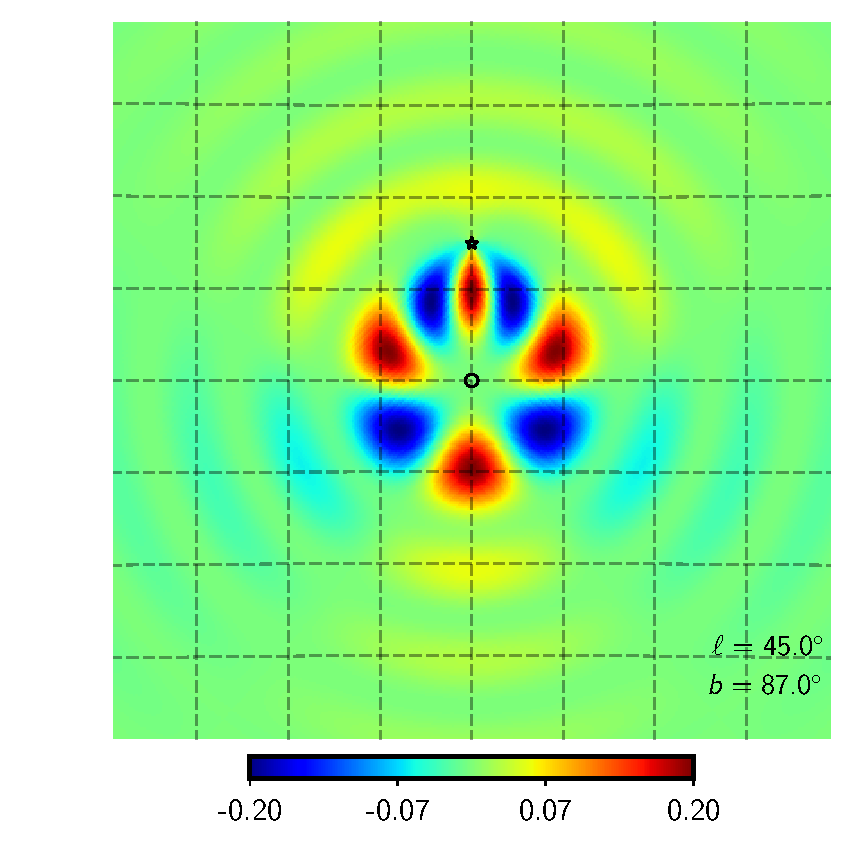
\includegraphics[width=0.125\columnwidth]{new_kernel/qu2ebqu_rker_D_lat87_lon45.pdf}}\hspace{-2mm}
%\subfigure{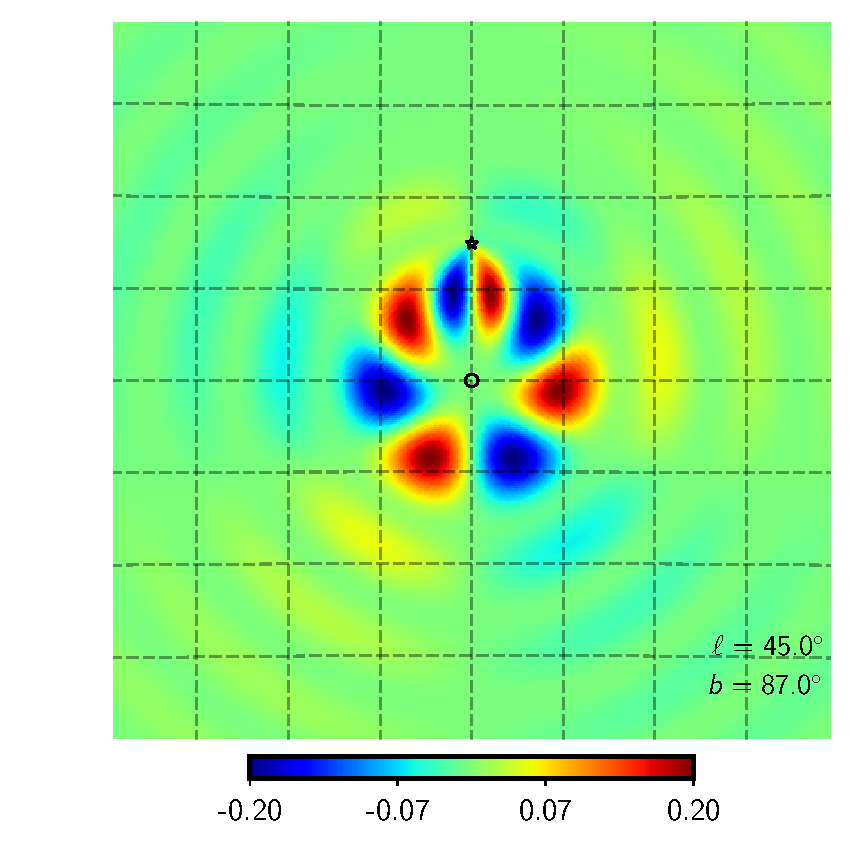
\includegraphics[width=0.125\columnwidth]{new_kernel/qu2ebqu_iker_D_lat87_lon45.pdf}}\hspace{-2mm}
%\subfigure{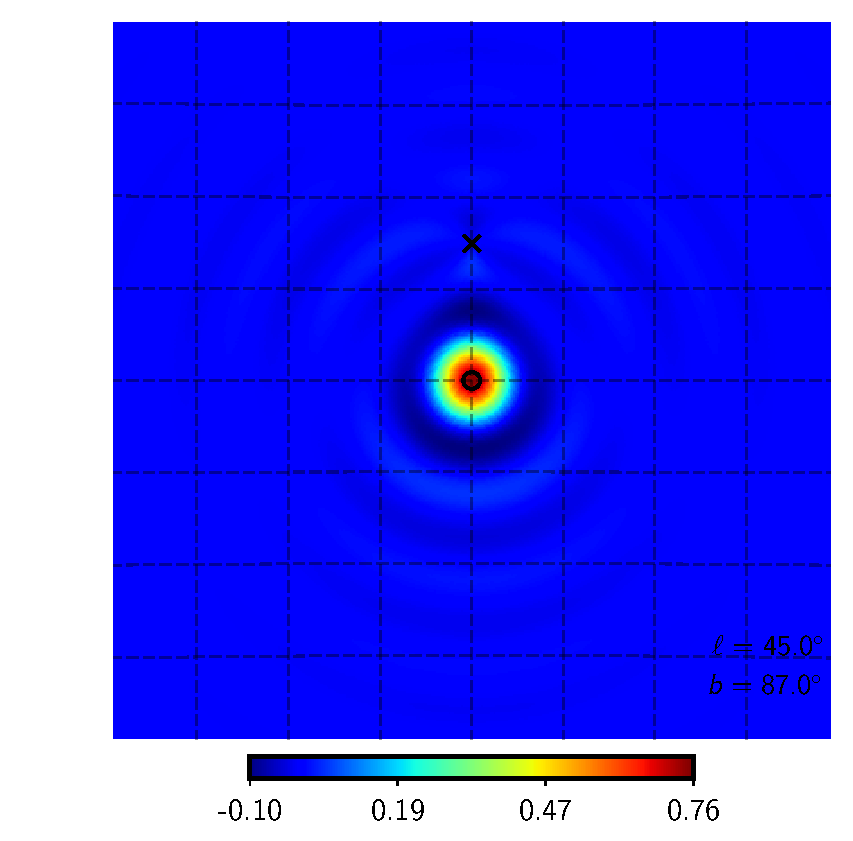
\includegraphics[width=0.125\columnwidth]{new_kernel/qu2ebqu_rker_I_lat87_lon45.pdf}}\hspace{-2mm}
%\subfigure{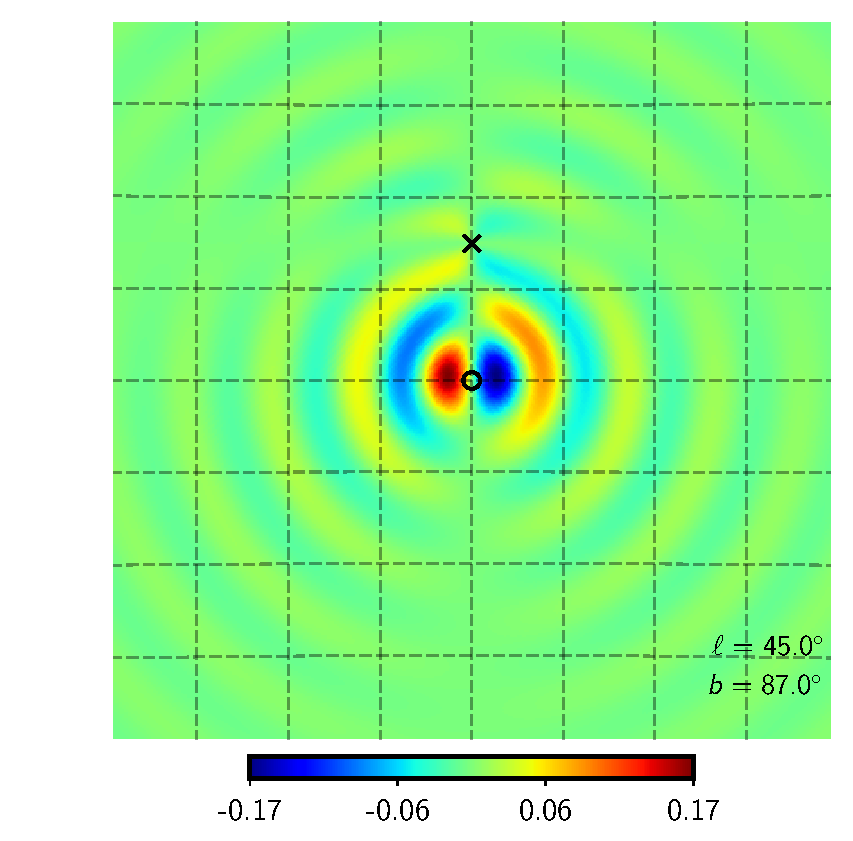
\includegraphics[width=0.125\columnwidth]{new_kernel/qu2ebqu_iker_I_lat87_lon45.pdf}}\hspace{-2mm}

%\subfigure{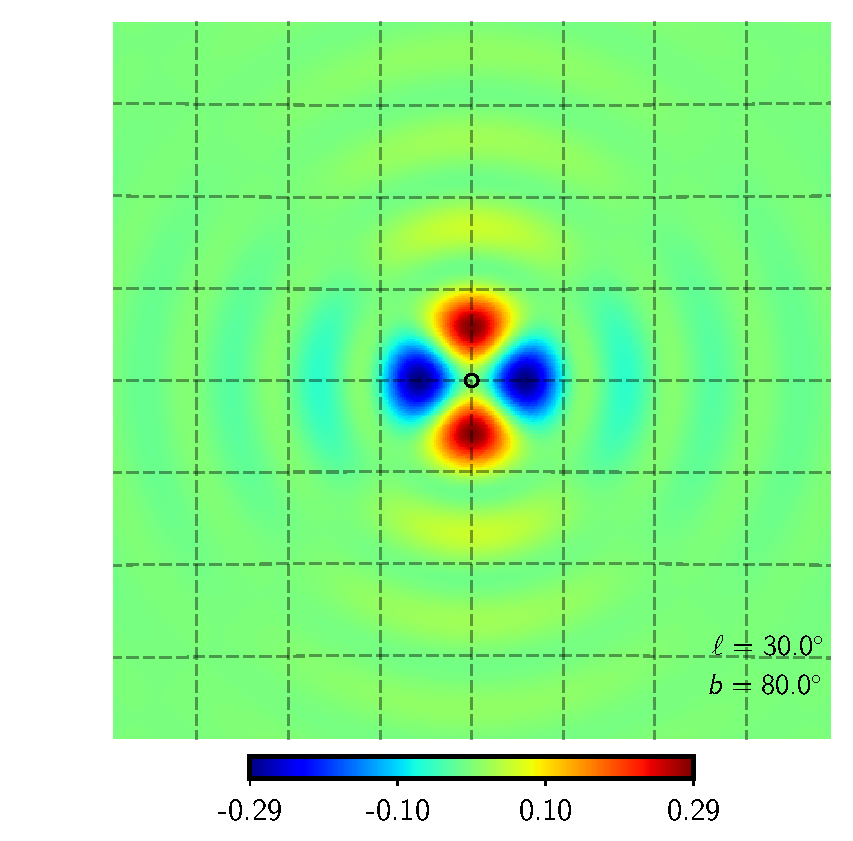
\includegraphics[width=0.125\columnwidth]{new_kernel/qu2eb_rker_rad_lat80_lon30.pdf}}\hspace{-2mm}
%\subfigure{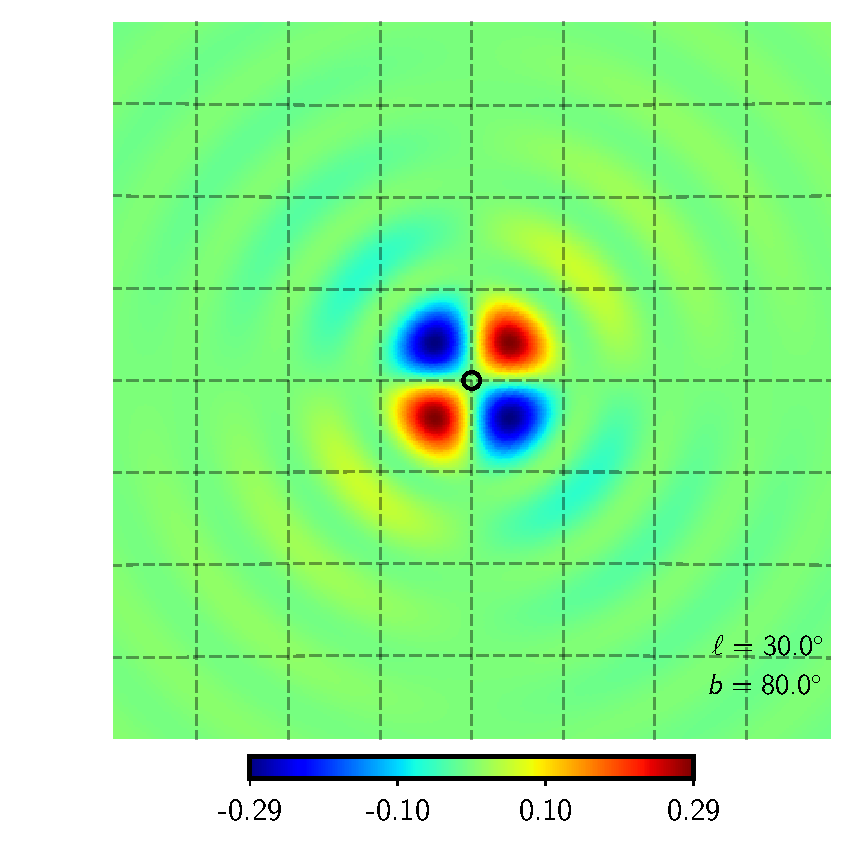
\includegraphics[width=0.125\columnwidth]{new_kernel/qu2eb_iker_rad_lat80_lon30.pdf}}\hspace{-2mm}
%\subfigure{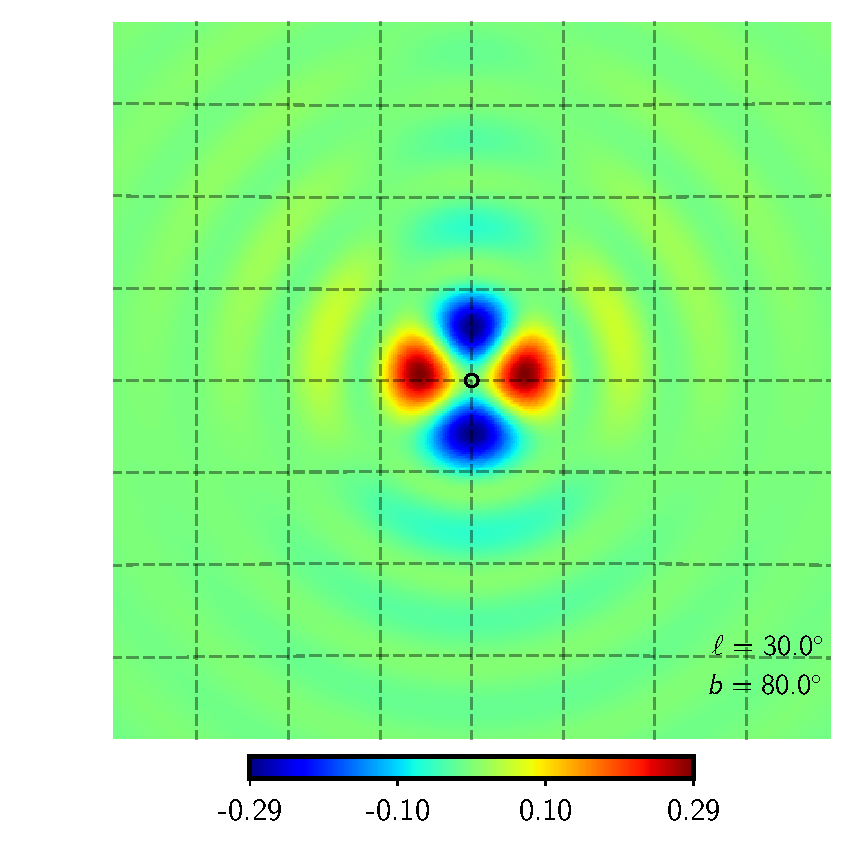
\includegraphics[width=0.125\columnwidth]{new_kernel/qu2eb_rker_con_lat80_lon30.pdf}}\hspace{-2mm}
%\subfigure{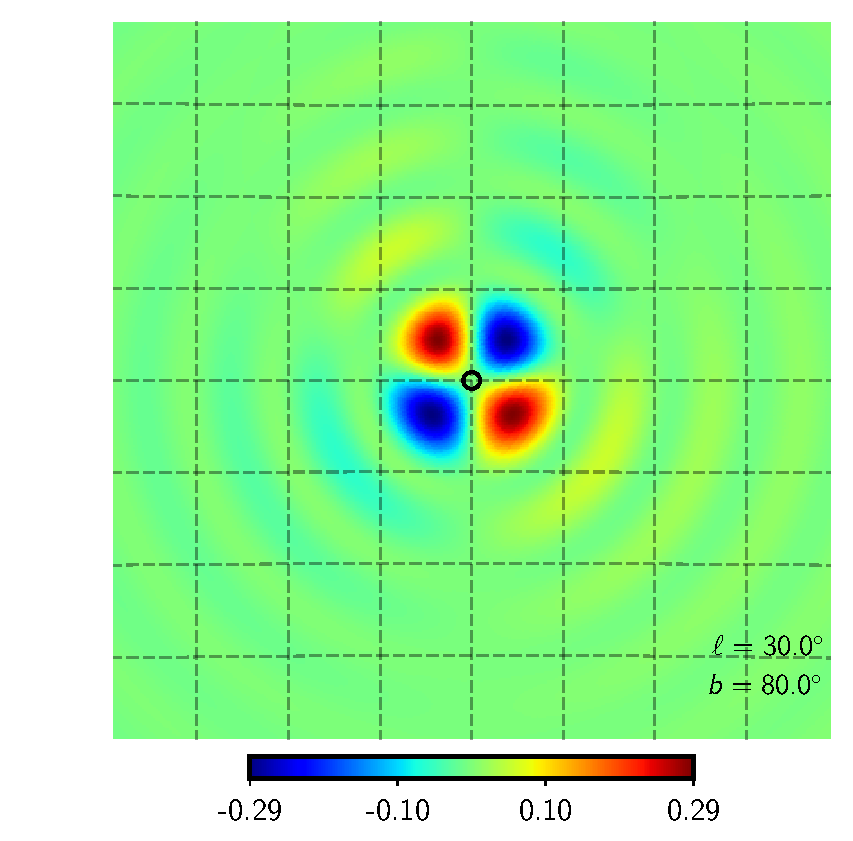
\includegraphics[width=0.125\columnwidth]{new_kernel/qu2eb_iker_con_lat80_lon30.pdf}}\hspace{-2mm}
%\subfigure{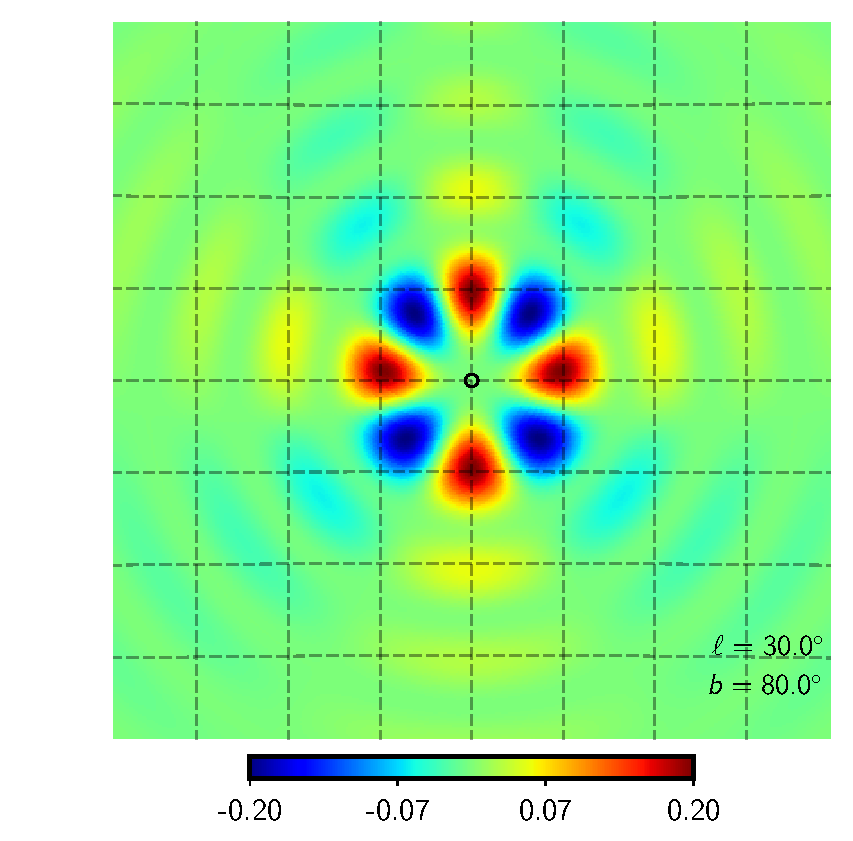
\includegraphics[width=0.125\columnwidth]{new_kernel/qu2ebqu_rker_D_lat80_lon30.pdf}}\hspace{-2mm}
%\subfigure{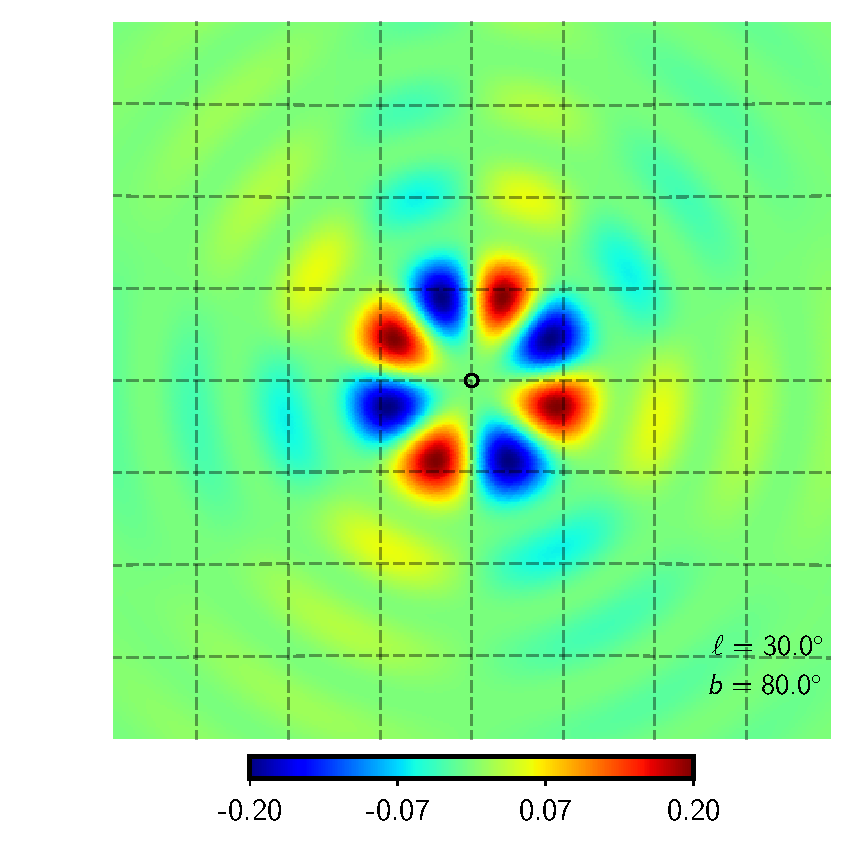
\includegraphics[width=0.125\columnwidth]{new_kernel/qu2ebqu_iker_D_lat80_lon30.pdf}}\hspace{-2mm}
%\subfigure{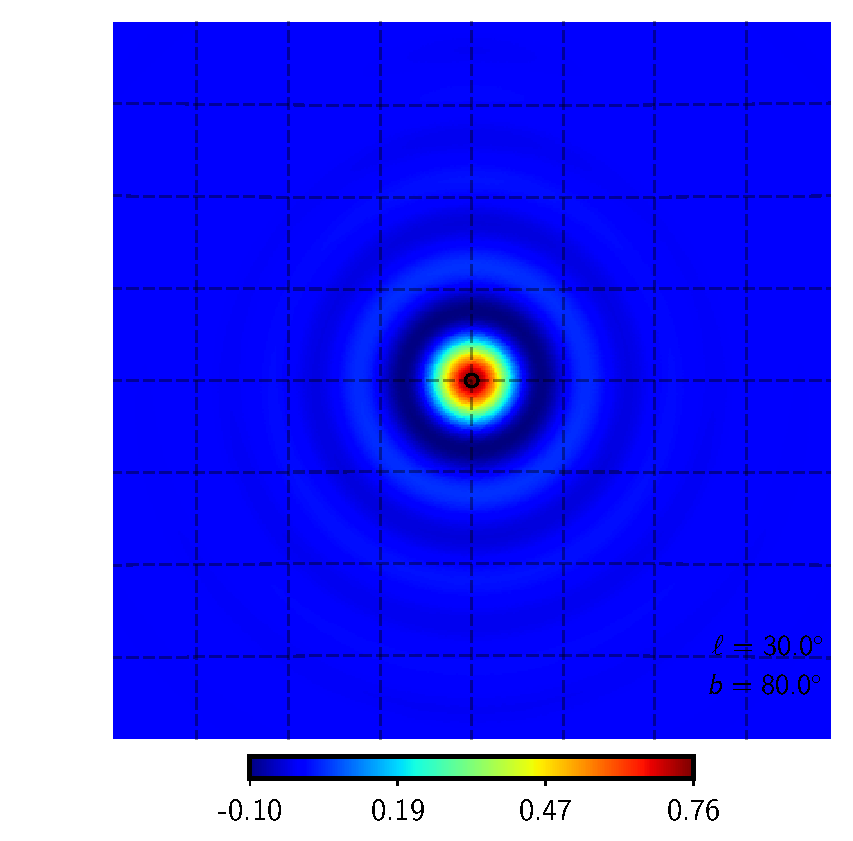
\includegraphics[width=0.125\columnwidth]{new_kernel/qu2ebqu_rker_I_lat80_lon30.pdf}}\hspace{-2mm}
%\subfigure{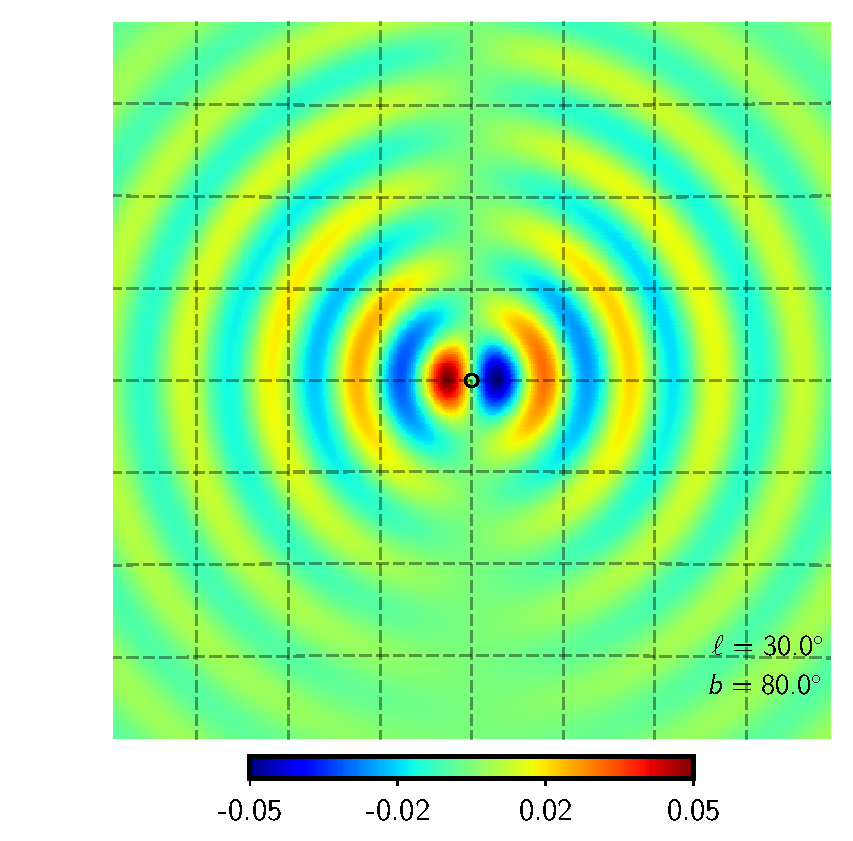
\includegraphics[width=0.125\columnwidth]{new_kernel/qu2ebqu_iker_I_lat80_lon30.pdf}}\hspace{-2mm}
%\subfigure[$ \textrm{Re} \left(\mathcal{M}_{G} \right) $]{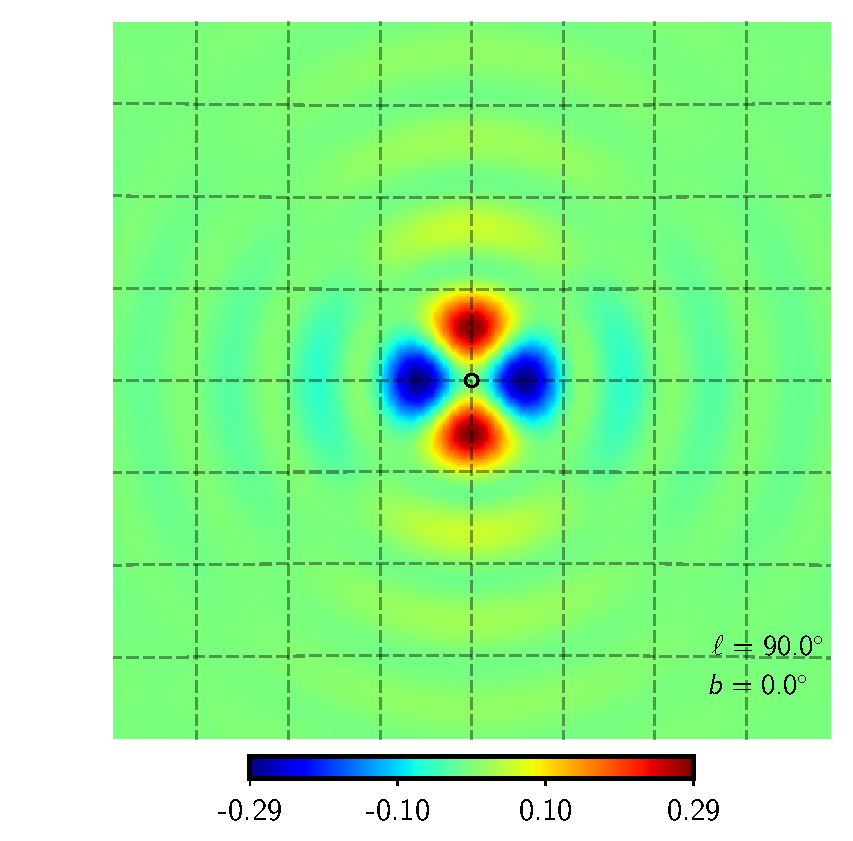
\includegraphics[width=0.125\columnwidth]{new_kernel/qu2eb_rker_rad_lat0_lon90.pdf}}\hspace{-2mm}
%\subfigure[$\textrm{Im} \left(\mathcal{M}_{G} \right) $]{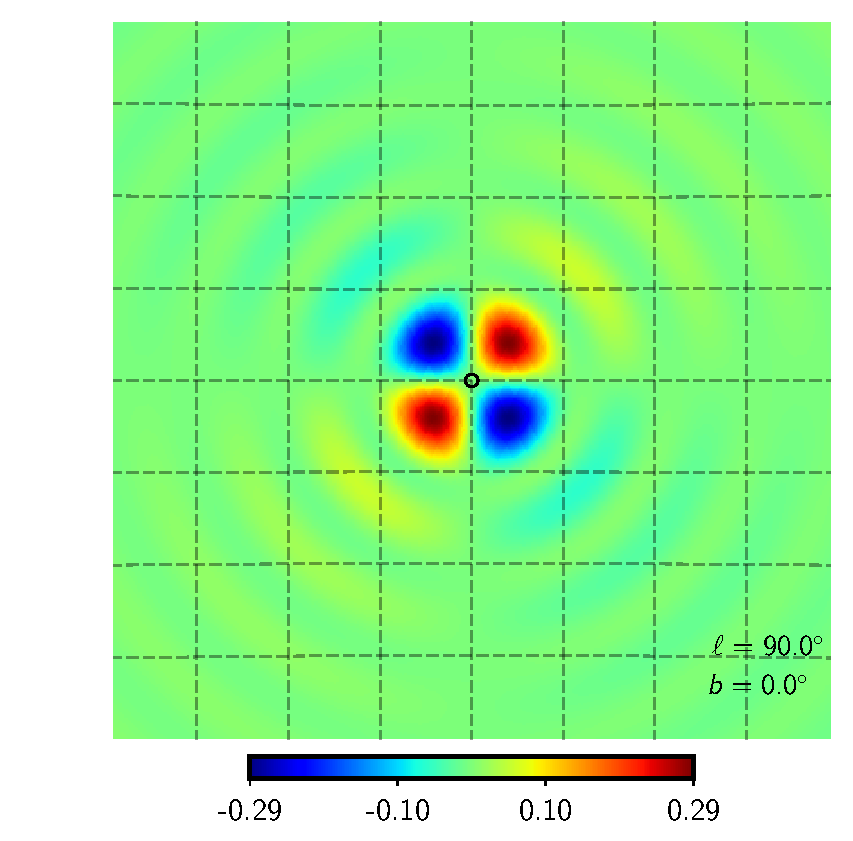
\includegraphics[width=0.125\columnwidth]{new_kernel/qu2eb_iker_rad_lat0_lon90.pdf}}\hspace{-2mm}
%\subfigure[$\textrm{Re}  \left(\mathcal{M}_{B}^* \right) $]{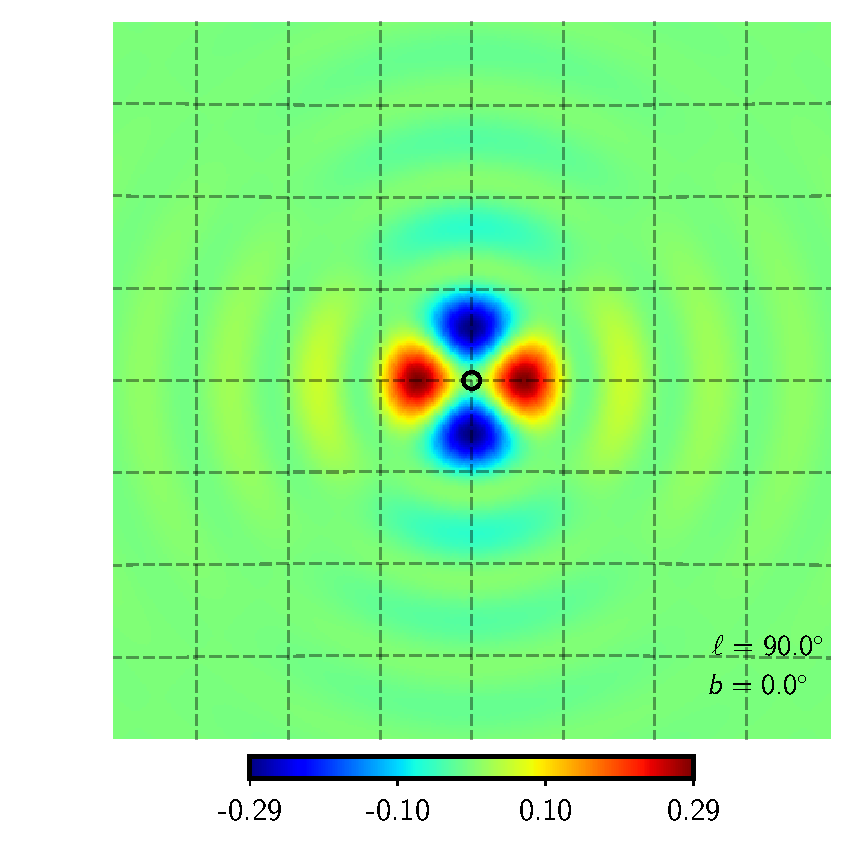
\includegraphics[width=0.125\columnwidth]{new_kernel/qu2eb_rker_con_lat0_lon90.pdf}}\hspace{-2mm}
%\subfigure[$\textrm{Im} \left(\mathcal{M}_{B}^* \right) $]{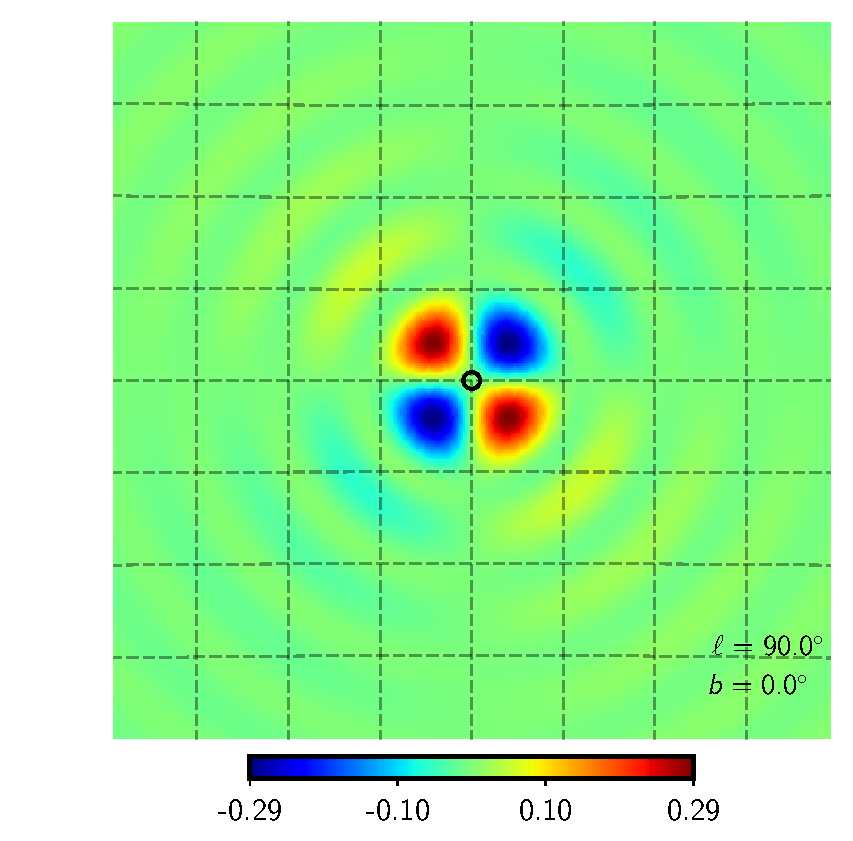
\includegraphics[width=0.125\columnwidth]{new_kernel/qu2eb_iker_con_lat0_lon90.pdf}}\hspace{-2mm}
%\subfigure[$\textrm{Re} \left(\mathcal{D} \right)$]{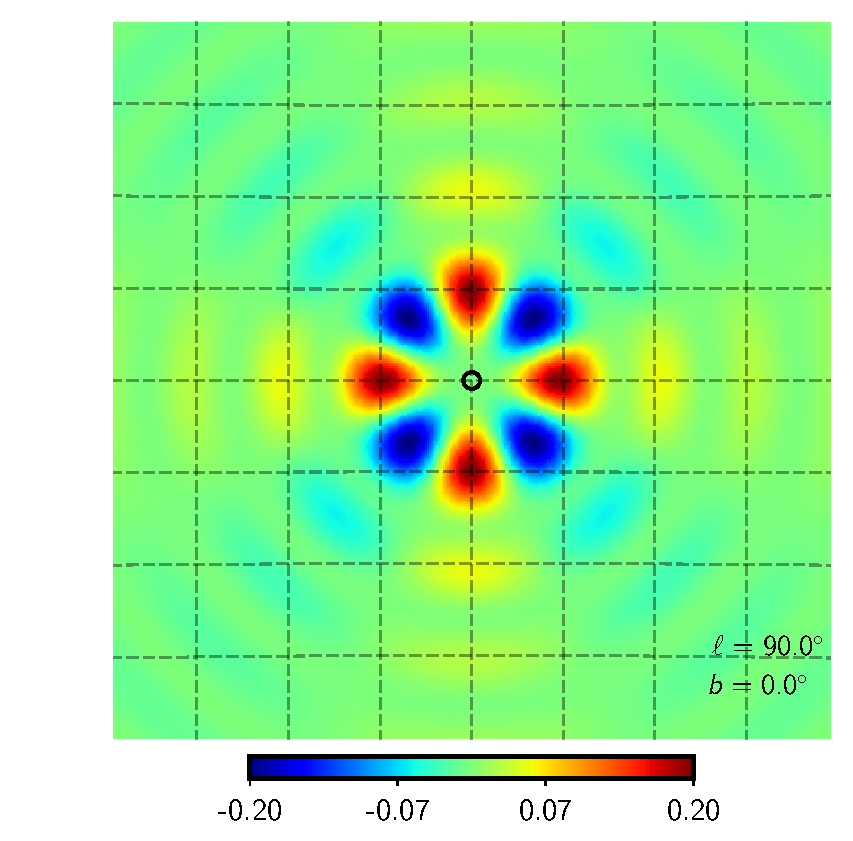
\includegraphics[width=0.125\columnwidth]{new_kernel/qu2ebqu_rker_D_lat0_lon90.pdf}}\hspace{-2mm}
%\subfigure[$\textrm{Im} \left(\mathcal{D} \right)$]{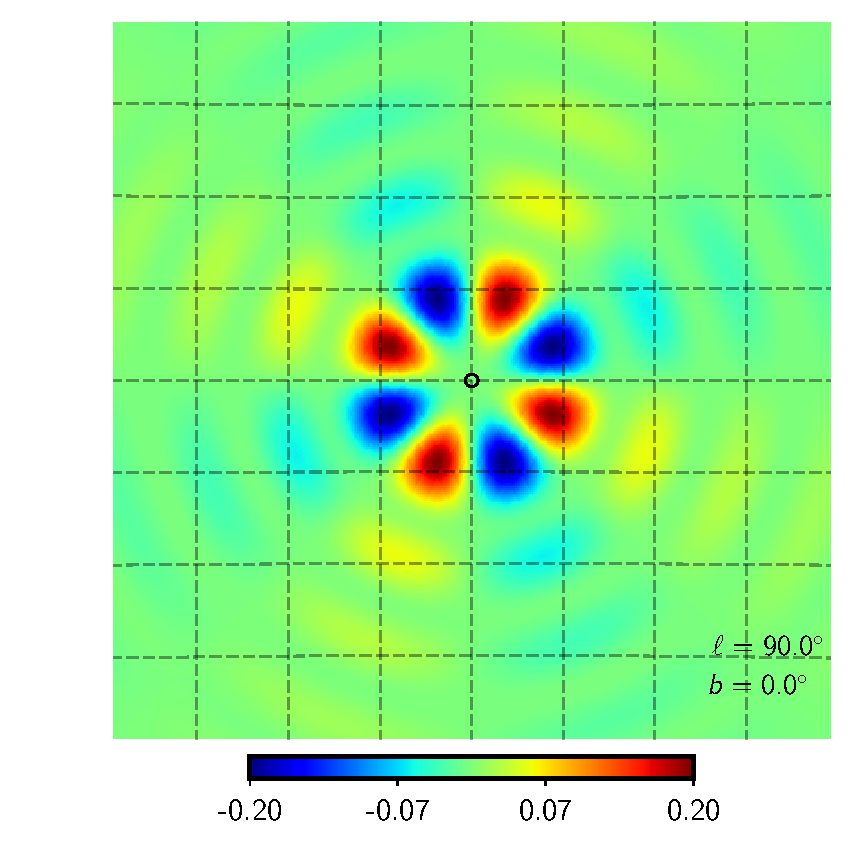
\includegraphics[width=0.125\columnwidth]{new_kernel/qu2ebqu_iker_D_lat0_lon90.pdf}}\hspace{-2mm}
%\subfigure[$\textrm{Re} \left(\mathcal{I} \right)$]{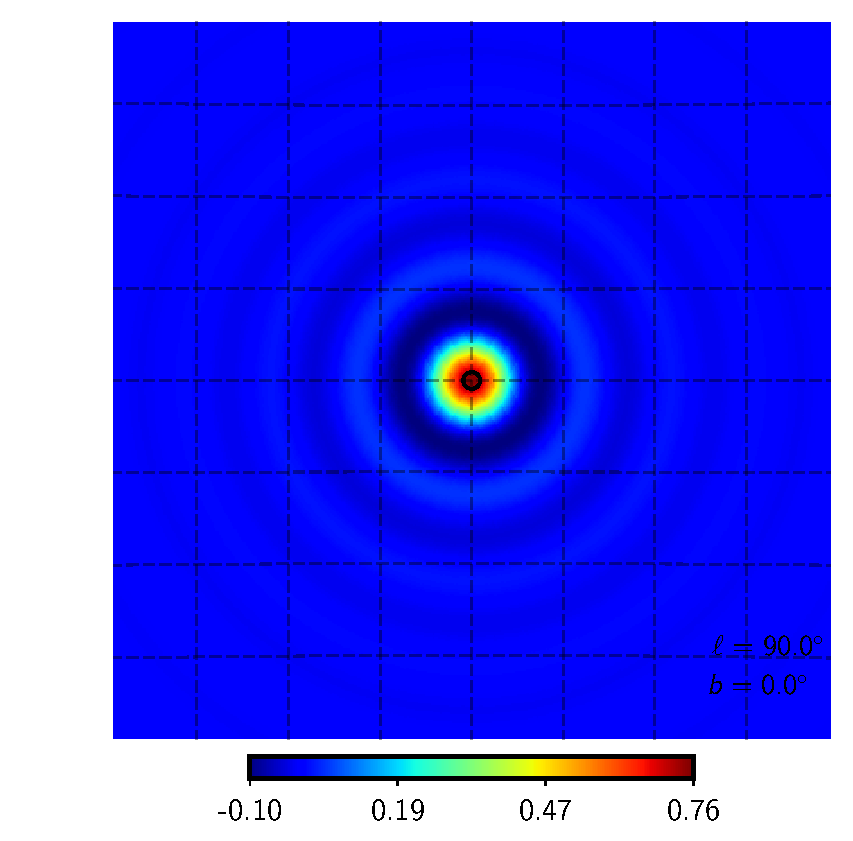
\includegraphics[width=0.125\columnwidth]{new_kernel/qu2ebqu_rker_I_lat0_lon90.pdf}}\hspace{-2mm}
%\subfigure[$\textrm{Im} \left(\mathcal{I} \right)$]{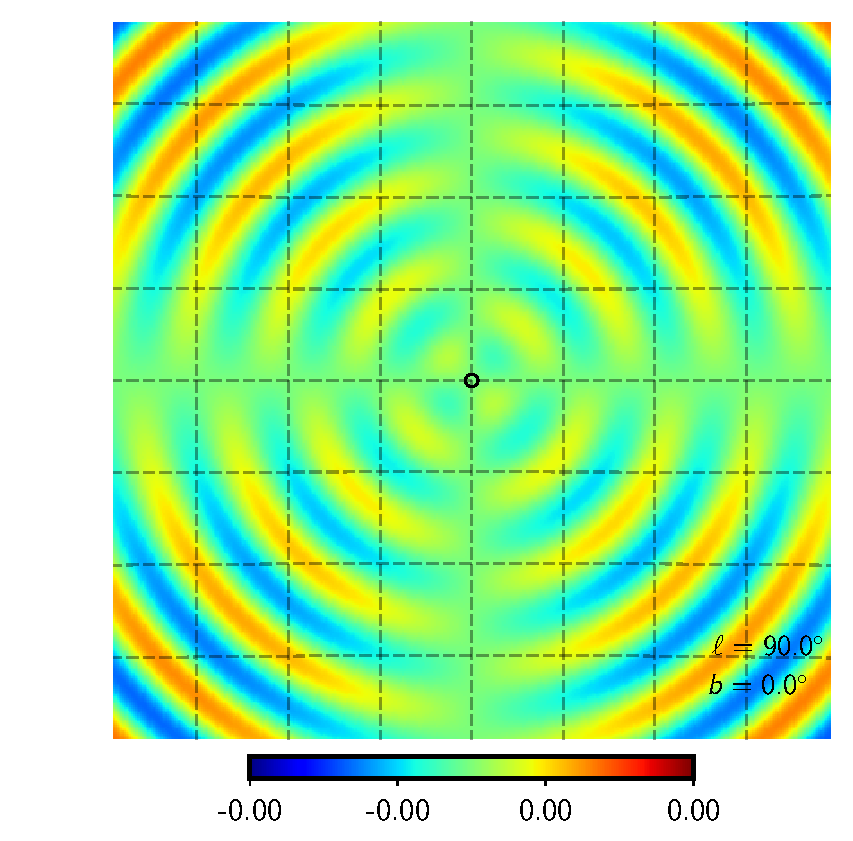
\includegraphics[width=0.125\columnwidth]{new_kernel/qu2ebqu_iker_I_lat0_lon90.pdf}}\hspace{-2mm}
%\caption{This panel of figure depicts the real and imaginary parts of the real space kernels $\mathcal{M}_{G}$, $\mathcal{M}_{B}$, $\mathcal{D}$ \& $\mathcal{I}$ respectively. These kernels have been evaluated with the band limit: $\ell \in [2,192]$ and sampled at the Healpix resolution parameter NSIDE=2048 for visual appeal. The size of each panel is approximately $16^{\circ} \times 16^{\circ}$ and the grid lines are marked at 2 degree separations. The black circles denotes the position of the center around which the kernels have been evaluated while the black star marks the location of the north galactic pole. The four rows depict the kernels at different location on the sphere and the galactic coordinates of the central pixel are specified in each panel.}
%from top to bottom rows are as follows $[b,\ell] = [0^{\circ},0^{\circ}], [87^{\circ},0^{\circ}], [87^{\circ},30^{\circ}], [80^{\circ},30^{\circ}], [0^{\circ},90^{\circ}]$.}
%\label{fig:vis_kernel}
% \end{figure}
%

%\textit{Evaluating the local kernels: }\revisit{Let us consider the case when one of the coordinates coincides with the north pole $\hat{z}=(0,0)$ (this refers to the point $\theta_0 \rightarrow 0$ while moving along the longitude $\phi_0=0$). In this case the Euler angles in the $z-y1-z2$ convention are simply given by: $(\alpha,\beta,\gamma) =(\phi_i,\theta_i,0)$, where $(\theta_i,\phi_i)$ denote the coordinates of the location $\hat{n}_i$.} Since the Euler angle $\gamma=0$ when rotations are defined with respect to the pole, the respective kernels simplify to the following forms,
%%
%\begin{subequations}
%\beqry 
%\mathcal{M}(\hat{z},\hat{n}_i) &=&  \sum_{\ell} {{}_{0}}a_{\ell 2} \, {{}_{0}}Y_{\ell 2}(\hat{n}_i) \,;\\
%\mathcal{I}(\hat{z},\hat{n}_i) &=& \sum_{\ell} {{}_{-2}}a_{\ell 2}\, {{}_{-2}}Y_{\ell 2}(\hat{n}_i) ~~\,;~~
%\mathcal{D}(\hat{z},\hat{n}_i) =\sum_{\ell} {{}_{2}}a_{\ell 2} \, {{}_{2}}Y_{\ell 2}(\hat{n}_i) \,,
%\eeqry
%\end{subequations}
%%
%where ${}_{s}a_{\ell 2} = \sqrt{\frac{2 \ell+1}{ 4 \pi}} ~~\forall ~~ s \in [0,-2,+2]$.
%The convolution kernels centered around any other location $\hat{n}_j = (\theta_j,\phi_j)$ are simply given by evaluating the respective spherical harmonic sums: $\sum_{\ell m} {}_{s}a_{\ell m}\,{}_{s}Y_{\ell m}(\hat{n}_i)$ using the rotated harmonic coefficients given by: ${}_s a_{\ell m} = D^{\ell}_{m 2}(\phi_j , \theta_j, 0) {{}_s}a_{\ell 2}$, where $D^{\ell}_{2 m}$ are the Wigner-D functions.
%These rotation operations can be carried out using inbuilt Healpix routine \textit{rotate\_alm}, while the convolution kernels can be synthesized by evaluating the respective spherical harmonic sums using the \textit{alm2map} routine. 
%\comment{Make parallels with instrument beam analysis here ? Or is it trivial since its obvious that all convolution problems can be cast in this form.}
 
%

The kernels $\mathcal{D}$ and $\mathcal{I}$ vary significantly as a function of galactic latitude of the central pixel, as seen in \fig{fig:vis_kernel_DI}. These kernels show a two fold symmetry in the vicinity of the poles.  Here the Euler angle $\gamma \approx 0$ here and therefore $e^{i2(\alpha \pm \gamma)} \approx e^{i2\alpha}$. Note that in this region, the azimuthal profile of the real and imaginary part of these kernels is identical to $-\mathcal{M}_G$.  The imaginary part of the band limited delta function $\mathcal{I}$ contributes just as much as the real part in these regions. On transiting to lower latitudes, however, $\mathcal{D}$ quickly transitions to having a four fold symmetry while $\mathcal{I}$ transitions to being dominated by the real part and behaves more like the conventional delta function. This transition can be most easily understood in the flat sky limit where $\gamma \approx -\alpha$ which leads to the resultant 4 fold symmetry seen for $\mathcal{D}$ owing to $e^{i2(\alpha - \gamma)} \approx e^{i4\alpha}$ and $\mathcal{I}$ being dominated by the real part owing to $e^{-i2(\alpha + \gamma)} \approx 1 + i0$. Since the flat sky approximation has most validity in the proximity of the equator these limiting tendencies of the respective kernels are seen in the bottom row of \fig{fig:vis_kernel_DI} which depict the kernels evaluated at the equator $b=0^{\circ}$. The middle two row depict the kernels evaluated at intermediate latitudes: $b=87^{\circ}$ and $b=80^{\circ}$ and serve to indicate the rate of this transition. As before, these kernels are invariant under changes in longitude of the central pixel with the latitude fixed.

%%%%%%%%%%%%%%%%%%%%%%%%%%%%%%%%%%%%%%%%%%%%%%%%%%%%%%%%%%%%%%%%%%%%%%%%%%
%\subsection{Quantifying the non-locality of E \& B modes} \label{sec:radial_locality}
\subsection{The non-locality of the real space operators} \label{sec:radial_locality}
%
\begin{figure}[t]
\centering
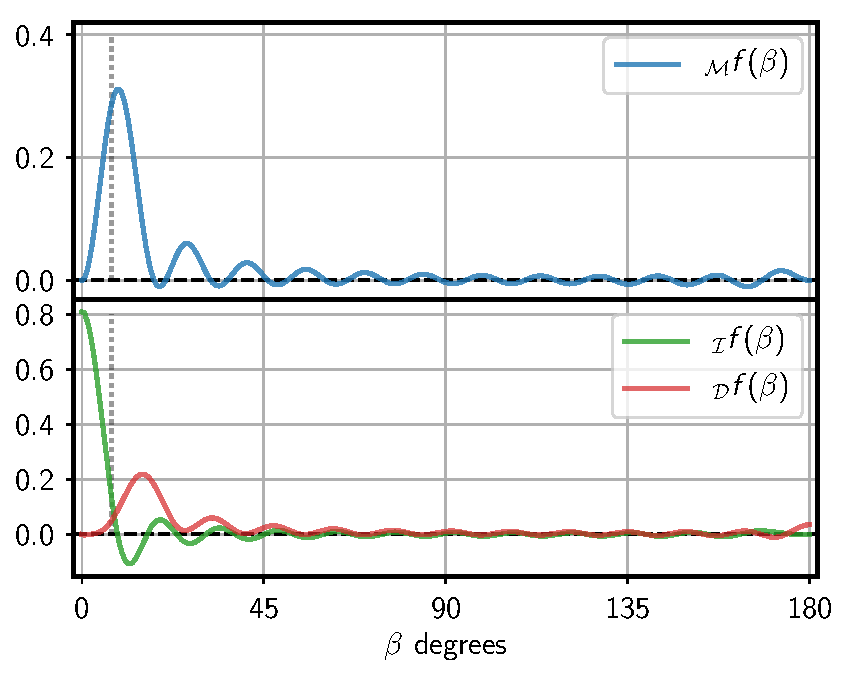
\includegraphics[width=0.8\columnwidth]{beta_kernel.pdf}
\caption{The figure depicts the radial part of the convolution kernels. These radial function have been evaluated with the band limit fixed at $\ell \in [2,24]$. The vertical dashed line marks the approximate Healpix pixel size of a NSIDE=8, which is the lowest resolution that allows access to $\ell_{\rm max}=24$.}
\label{fig:beta_kernel}
\end{figure}
%
Above, we have explored in detail the  azimuthal dependence of the real space kernels.  Here we probe the radial dependence, which both  determines the non-locality of the operators and encodes all their multipole dependencies. For illustration, \fig{fig:beta_kernel} shows the radial kernels ${_{\mm}f}, {_{\md}f},{_{\mi}f}$, evaluated using the respective multipole sums given in \eq{eq:rad_ker_queb} and \eq{eq:f2_rad_ker} in the band limit $\ell \in [2,24]$. We choose a low band limit to evaluate these radial kernels to highlight some key features of their radial profile.
%
\begin{figure}[t]
\subfigure[\label{fig:fbeta}]{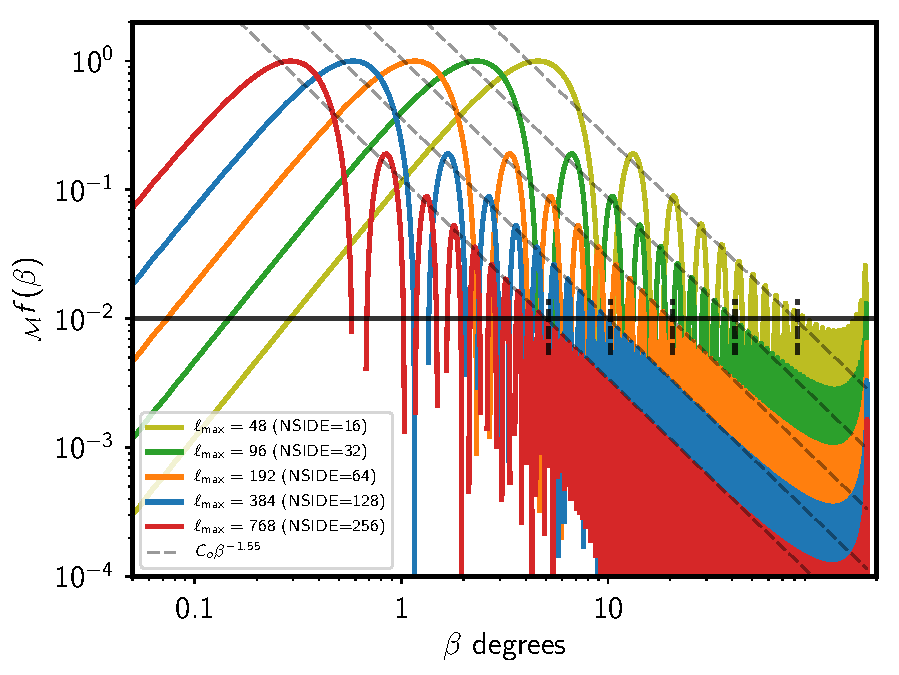
\includegraphics[width=0.325\columnwidth]{rad_ker_fn_of_ellmax.pdf}}\hfill
\subfigure[\label{fig:dfbeta}]{\includegraphics[width=0.325\columnwidth]{rad_ker_d_fn_of_ellmax.pdf}}\hfill
\subfigure[\label{fig:ifbeta}]{\includegraphics[width=0.325\columnwidth]{rad_ker_i_fn_of_ellmax.pdf}}\hfill
\centering
\subfigure[\label{fig:fbeta_avg}]{\includegraphics[width=0.325\columnwidth]{rad_ker_fn_of_ellmax_zaldariagga_scaling.pdf}}
\subfigure[\label{fig:dfbeta_avg}]{\includegraphics[width=0.325\columnwidth]{rad_ker_i_fn_of_ellmax_zaldariagga_scaling.pdf}}

\caption{This figures depicts the radial functions for the different kernels and varying band limit set by fixed $\ell_{\rm min}=2$ and varying $\ell_{\rm max}$ as indicated by their legends. \fig{fig:fbeta} depicts ${_{\mm}f}(\beta,\ell_{\rm min},\ell_{\rm max})$, \fig{fig:dfbeta} depicts ${}_{\md}f(\beta,\ell_{\rm min},\ell_{\rm max})$ and  \fig{fig:ifbeta} depicts ${}_{\mi}f(\beta,\ell_{\rm min},\ell_{\rm max})$ respectively. All the curves are normalized such that their maxima is set to unity. The horizontal solid black line marks the location where the amplitude of the respective kernels fall below 1\% of its maximum. The thin slanted dashed gray lines indicate a power law fit (by eye) to the envelope of the radial functions. The thick black short vertical dashed lines indicate the transition points as predicted by the empirically derived relation for the non-locality parameter $\beta_0={\rm min}(180^\circ,180^\circ \times 22/\ell_{\rm max})$. \fig{fig:fbeta_avg} and  \fig{fig:dfbeta_avg} depict the radial functions $\langle{_{\mm}f}(\beta,\ell_{\rm min},\ell_{\rm max})\rangle$ and $\langle{_{\md}f}(\beta,\ell_{\rm min},\ell_{\rm max})\rangle$ respectively where $\langle \cdots \rangle$ denotes a moving average over a step function centered at $\beta$ and has width $1.4\beta_0$. These smoothed functions are seen to be well fit by a power law $\propto \beta^{-2}$  and depict the average radial response.}
%While the envelopes for function ${_{\mm}f}(\beta)~\&~ {}_{\mi}f(\beta)$ are fit well by the power law $\propto \beta^{-1.5}$, the envelope for the function ${}_{\md}f(\beta)$ is seen to have a slightly steeper slope $\propto \beta^{-1.65}$.}
\label{fig:rad_ker_decay}
\end{figure}
%

The function ${_{\mm}f}$ is the radial part of the kernel that translates the Stokes parameters $Q$/$U$ to scalars $E$/$B$ and vice versa.  It oscillates and as a consequence of the spin-2 symmetry, it vanishes as $\beta \rightarrow 0$ and $\beta \rightarrow \pi$, since the Euler angles $\alpha$, $\gamma$ are not uniquely defined at those separations.
%This nature of ${_{\mm}f}$ is critical to ensure that the derived fields have the necessary spin properties.

The radial part of the kernel that decomposes the  Stokes parameters into parts that correspond to $E$ and $B$ modes  are also  necessarily non-local.  The function ${_{\mi}f}$ is the radial part of the band limited delta function $\mi$.  It expectedly has its maxima at $\beta=0$ and decays with increasing angular separation.  ${_{\md}f}$ has a vanishing value in the region where $\beta \rightarrow 0$ however it does not vanish at $\beta \rightarrow \pi$ as seen in \fig{fig:beta_kernel}.

\paragraph{Band limit dependence.} 
%It is clear from previous discussions that the scalar field $E$ \& $B$ constructed at a location depends on the Stokes field in the surrounding regions. 
To quantify this non-locality, we study the radial extent of the kernels and its dependence on the maximum multipole accessible. We evaluate the radial functions for different values of $\ell_{\rm max}$, while keeping the lowest multipole fixed at $\ell_{\rm min}=2$. 

The resultant set of radial function are depicted in \fig{fig:rad_ker_decay}. While the amplitude of these radial function scales up as $\propto \ell_{\rm max}^2$, for clarity in the plot their global maxima are normalized to unity.  This normalization highlights the key feature, that on increasing $\ell_{\rm max}$ the radial kernels shift left, attaining their global maxima at progressively small angular distances $\beta$.  At intermediate values of $\beta$, the envelope of the radial functions is fit well by a power law $ \propto \beta^{-n}$ as seen in \fig{fig:rad_ker_decay}.
In fact these finding are neatly summarized in the observation that the radial functions computed by evaluating the multipole sums to different maximum multipoles are approximately self-similar and follow this telescoping and scaling property: $${}_rf(\beta,2,\ell_{\rm max}) \approx \Big[\frac{\ell_{\rm max}}{\ell'_{\rm max}}\Big]^2{}_rf(\beta'=\frac{\ell'_{\rm max}}{\ell_{\rm max}} \beta ,2,\ell'_{\rm max}) \,,$$ where ${}_rf , r \in [\mm, \md,\mi]$ denotes all the different radial functions. We can now understand the amplitude scaling and the shifting left of the radial kernels on increasing the maximum multipole by studying this telescoping property. Specifically the global maxima of the kernel with maximum multipole $\ell_{max}$ is amplified/supressed by a factor $(\ell_{\rm max}/\ell'_{\rm max})^2$ and the oscillating part is compressed/expanded by a factor $(\ell'_{\rm max}/\ell_{\rm max})^{-1}$ with respect to the kernel defined by the maximum multipole $\ell'_{\rm max}$.

To quantify the non-locality of the scalar modes $E/B$, we can define a characteristic angular radius of the region from which the kernels get most of their contribution.   We define a non-locality parameter $\beta_{0}$ as the angular distance beyond which the function ${_{\mm}f}(\beta,\ell_{\rm min}=2,\ell_{\rm max})$ transitions to being consistently below 1\% of its maximum.
%For $\ell_{\rm max}=24$, the maximum multipole accessible on a Nside=8 Healpix map, the non-locality parameter $\beta_0=180^{\circ}$ as the radial function never falls monotonously below 1\% of its global maxima as seen in \fig{}. Using this fact and the self similar property of the radial functions, we define the following empirical relation: $\beta_o= {\rm min}(180,180 \frac{24}{\ell_{\rm max}})$, as a means of estimating the non-locality parameter given the maximum multipole $\ell_{\rm max}$ accessible for analysis.
The empirical relation:
\beq
\beta_0= {\rm min}\left(180^\circ,180^\circ \frac{\ell_{0}}{\ell_{\rm max}} \right) \,,
\eeq
with $\ell_{0}=22$ provides a reasonable estimate of this transition point for ${}_{\mm}f$ as seen in \fig{fig:rad_ker_decay}. Setting $\ell_{0}=10$ and $\ell_{0}=32$ predicts the transition points for the functions ${}_{\mi}f$ and  ${}_{\md}f$ respectively.%\comment{How sensitive is this transition point to $\ell{\rm min}$?} 

\revisit{In the flat sky limit it has been argued that form of the radial function has to be ${}_\mm f(\beta)\simeq\beta^{-2}$ so as to ensures that the Fourier modes for Stokes parameters $Q/U$ are related  to those of $E/B$ modes merely by rotations and no scale dependent factor \cite{Zaldarriaga2001a}. Here we numerically studied the formally derived radially function ${}_\mm f(\beta)$ which reveals an oscillatory nature with amplitude decaying on increasing angular distance. While we find that the positive envelope of ${}_{\mm}f$ scales as $\beta^{-1.55}$, the function resulting from performing a sliding average on it is seen to scale as $\beta^{-2}$ at intermediate angular separations as seen in \fig{fig:fbeta_avg}, in agreement with the hypothesis made in \cite{Zaldarriaga2001a}. We find that the function resulting from performing a sliding average on ${}_{\md}f$ also shows a similar scaling of $\beta^{-2}$ as seen in \fig{fig:dfbeta_avg}.}

\revisit{In essence the radial function resulting from taking a sliding average can be thought of as transitioning to some lower band limit (determined by the width of the sliding window) radial function from a higher band limit radial function.  On carrying out this moving average on radial functions evaluated with a progressively increasing band limit, one seen that a larger fraction of the radial function matches the scaling of $\beta^{-2}$. Extrapolating this trend to the case of infinite band limit one can see that the behaviour will approach $\beta^{-2}$ across the domain $\beta\in[0,\pi]$.}

\revisit{Near the edges of the domain $\beta \rightarrow 0,\pi$ the window function gets modified and is partly responsible for the scaling deviating from the power law. More importantly note that ${}_{\mm}f$ and ${}_{\md}f$ vanish at $\beta=0$ and therefore the sliding average in the vicinity of this point cannot have a power law behaviour of the form $\beta^{-2}$.}
